


\tableofcontents

%\emptypage
\newpage

\chapternonum{Introduction}

%==============================================================
\chapter{The Standard Model of particle physics and beyond}
%==============================================================

    \section{Fields and symmetries}

        \subsection{Quantum field theory and feynman diagrams}


	While the topic of interest here is the physics of particles, one should 
    never forget about the underlying structure behind them : fields. A field 
    is a physical quantity defined across space and time. Relative quantum 
    field theory is a theoretical framework which was developed during the 
    twentieth century and allowed to unify quantum mechanics and special 
    relativity.

	In such a field theory, particles are excitations of the fields (of field 
    quanta) and interactions refers to coupling terms between those fields. 
    In a sense, the goal of a particle physicist can be seen as using particles
    as a mean to understand which fields exists, what are their properties and
    how they couple with each other.

    Quantum field theory makes use of the Lagrangian formalism. In particular, 
    the Lagrangian function $\mathcal{L}$ is a core element as it allows to 
    summarize the dynamics of a system in an elegant and concise way. This 
    function depends of the fields $\phi(t,x)$ and their derivatives with 
    respect to time and space. One can obtain the equation of motion from it 
    by using the Euler-Lagrange equation :

    $$
        \frac{\partial \mathcal{L}}{\partial \phi} 
        - 
        \frac{\partial}{\partial x^\mu} 
        \left( 
            \frac{\partial \mathcal{L}}{\partial (\partial \phi / \partial x^\mu)} 
        \right) 
        = 
        0
    $$

    An interesting feature of the Lagrangian is that terms that are a product
    of three of more fields corresponds to an interaction between these fields.
    For instance in the simple case with three scalar fields $\phi_{i,\ i = 1,2,3}$, 
    a term $k \cdot \phi_1 \phi_2 \phi_3$ corresponds to a coupling between those
    fields with a strength $k$. 
    
    There is also a direct correspondance between such a term and an interaction 
    vertex which can be represented using Feynman diagram. Feynman diagrams are 
    graphical representations of the evolution of a system of particles where 
    interactions occur. Though there is no general convention about the orientation 
    of space and time when drawing such a diagram, this document will always 
    represent space along the horizontal axis and time evolving from left to right.
    Feynman diagrams provides an intuitive understanding of a physical process but 
    also a mathematical tool to compute probility amplitude for a transition between 
    an initial state and a final state using Feynman rules.

    \insertFigure{feynmanDiagramExample}{0.3}
                 {Example of vertex corresponding to a Lagrangian term $k \cdot \phi_1 \phi_2 \phi_3$.}

        \subsection{Noether's theorem and symmetries}
        \loremipsum

    \section{The Standard Model of particle physics}
        \subsection{The strong sector}
        \loremipsum
        \subsection{The electroweak sector}
        \loremipsum
        \subsection{The electroweak symmetry breaking}
        \loremipsum

    \section{Limitations of the Standard Model}
        \subsection{Open questions and criticism}
        \loremipsum
        \subsection{The hierachy problem}
        \loremipsum
        \subsection{The dark matter}
        \loremipsum

    \section{Theories beyond the Standard Model}
        \subsection{Zoology of Standard Model extensions}
        \loremipsum
        \subsection{Supersymmetry}
        \loremipsum
        \subsection{Constrains on top partners and dark matter}
        \loremipsum
            \subsubsection{Cosmology}
        \loremipsum
            \subsubsection{Particle physics}
        \loremipsum











%==============================================================
\chapter{The Compact Muon Solenoid experiment at the LHC}
%==============================================================

    \section{The Large Hadron Collider}
        \loremipsum
        \subsection{Scientific context and program}
        \loremipsum
        \subsection{Setup}
        \loremipsum
        \subsection{Performances during Run I}
        \loremipsum

    \section{The Compact Muon Solenoid experiment}
        \loremipsum
        \subsection{The CMS detector}
        \loremipsum
            \subsubsection{The tracker and magnet}
        \loremipsum
            \subsubsection{The calorimeters}
        \loremipsum
            \subsubsection{The muon chambers}
        \loremipsum
        \subsection{Trigger system}
        \loremipsum
            \subsubsection{L1}
        \loremipsum
            \subsubsection{HLT}
        \loremipsum
        \subsection{Object reconstruction algorithms and calibration}
            \subsubsection{Vertex and tracks}
        \loremipsum
            \subsubsection{Electrons and photons}
        \loremipsum
            \subsubsection{Muons}
        \loremipsum
            \subsubsection{Jets and missing energy}
            %(maybe plot showing the difference of jet clust algorithm for a same event/example)
        \loremipsum
        \subsection{Performances}
        \loremipsum
            \subsubsection{Particle-flow vs Calo-based algorithm ?}
        \loremipsum
            \subsubsection{Expected vs current performances ?}
        \loremipsum
            \subsubsection{Upcoming upgrades ?}
        \loremipsum

     \section{Monte Carlo generator and detector simulation}
        \loremipsum
        \subsection{Hard scattering}
        \loremipsum
        \subsection{Parton showering}
        \loremipsum
        \subsection{Detector simulation}
        \loremipsum

%==============================================================
\chapter{b-tagging techniques in CMS}
%==============================================================

    \section{Principle and importance of b-tagging techniques}
        \loremipsum

    \section{Discriminating observables and algorithms}
        \loremipsum
        \subsection{Impact parameter}
        \loremipsum
        \subsection{Secondary vertex}
        \loremipsum
        \subsection{Soft leptons}
        \loremipsum
        \subsection{Track counting algorithm}
        \loremipsum
        \subsection{Simple secondary vertex}
        \loremipsum
        \subsection{CSV}
        \loremipsum

    \section{Algorithms performances and prospectives}
        \loremipsum
        \subsection{Performances at 8 TeV}
        \loremipsum
        \subsection{Expected performances for Run II}
        \loremipsum
        \subsection{Development of boosted algorithms}
        \loremipsum
        \subsection{Studies for high PU conditions}
        \loremipsum







%==============================================================
\chapter{Search for stop pair production at $\sqrt{s}$ = 8 TeV}
%==============================================================

    This chapter focuses on an analysis performed within the CMS collaboration 
    and searching for the production of stop pair using the data recorded during 
    the Run I of the LHC at $\sqrt{s}$ = 8 TeV. In section \ref{sec:analysis_contextAndPheno}, 
    we concentrate on the context and phenomelogy of the signature while section 
    \ref{sec:analysis_objectAndEventSelection} to \ref{sec:analysis_results} discuss 
    the different aspects of the analysis itself and the results. In the last sections 
    \ref{sec:analysis_perspective} and \ref{sec:analysis_overviewStopSearches}, some 
    of the perspectives for this analysis are presented, as well as an overview of 
    other top-partner searches within the CMS collaboration.

    \section{Context and phenomenology \label{sec:analysis_contextAndPheno}}

        \subsection{Theoretical context and assumptions}

        One of the best assets of supersymmetry is its ability to explain the low mass
        of the Higgs boson, since the boson-fermion symmetry introduces a mechanism to
        protect the mass of the Higgs . This is illustrated on Figure
        \ref{fig:higgsCorrections}, showing the one-loop corrections to $m_H^2$
        from a fermionic and bosonic field coupled to the Higgs via the Lagrangian terms
        $- \lambda_f H \bar{f} f$ and $\lambda_b \left| H \right|^2 \left| b \right|^2$.
        \todo{cite S Liem somewhere here}. The leading order corrections writes :

        \insertFigure{higgsCorrections}{0.8}
                     {\todo{redo figure} One-loop correction to the Higgs for a fermionic field $f$ and bosonic field $b$.}

        \begin{equation}
            \Delta \mass{h}^2 = - \frac{\left| \lambda_f \right|^2}{8\pi^2} \Lambda^2_{\text{UV}}
            \, \, \, \, \, \, \, \, \, \, \text{and} \, \, \, \, \, \, \, \, \, \,
            \Delta \mass{h}^2 =   \frac{\lambda_b}{16\pi^2} \Lambda^2_{\text{UV}}
        \end{equation}

        where $\Lambda^2_{\text{UV}}$ is the ultraviolet momentum cutoff which regulates
        the loop integral. In the most ideal case, one could have $\left| \lambda_f \right|^2
        = \lambda_b$ and associate two scalar to each fermion (one for each chirality), 
        the corrections cancel each others. \todo{should clarify link between $\lambda$ and masses..}
        This however does not happens if the mass of the particle and its superpartner 
        are not the same, and tunning has to be reintroduced to keep the Higgs mass low.
        This is especially important in the case of the top as the correction it introduces
        on $\mass{h}^2$ is one of the biggest. 
        
        One can estimate the level of tunning needed as function of the superpartner of
        the top for the theory to keep providing a natural explanation to the hierarchy
        problem, and use it as a constrain. Despite the fact that such constrain is 
        highly dependent of hypothesis made on the SUSY parameters, it is commonly admitted 
        that stop quarks should have a mass below or around 1 TeV for SUSY to remain natural.
        This makes the search for stop and important channel for possible SUSY discovery.

        A second appealing feature of supersymmetry is that it can provide a dark matter 
        candidate. This happens in R-parity conserving models where the lightest supersymmetric
        particle (LSP) is a natural WIMP candidate if it is not a charged particle. In the
        context of the MSSM, the lightest neutralino $\lneutralino$, the gravitino $\tilde{G}$
        and the lightest sneutrino $\tilde{\nu}$ can be the LSP and therefore are dark matter
        candidate. The lightest neutralino is the one that is most often studied. Neutralinos
        $\tilde{\chi}$ are combination of the bino $\tilde{B}$, the two neutral higgsinos 
        $\tilde{H}_{1,2}$, and the neutral wino $\tilde{W}_3$. One can compute the relic
        abudance of dark matter by solving the Boltzmann equation \cite{EllisDarkMatter}
        depending essentially of the LSP mass $m_{\text{LSP}}$ and the annihilation cross-section.
        The next-to-lightest supersymmetric particle (NLSP) mass is a crucial parameter as 
        it strongly affect the annihilation cross-section and therefore the relic abudance. 
        In particular, cosmological observations are favorizing cases where the LSP is 
        degenerated with the lightest stop $\lstop$ or stau $\tilde{\tau_1}$.
        
        These two considerations lead to a logical interest in phenomenology where both a 
        neutralino LSP and a light stop NLSP have relatively low mass and accessible at the LHC.

        \subsection{Phenomenology and signature}

        In this subsection, we focus on presenting the targetted process of the search discussed 
        in sections \ref{sec:analysis_objectAndEventSelection} to \ref{sec:analysis_results} and 
        its phenomenology. As it is in practice impossible to scan the whole phase space of SUSY
        models, a pragmatic approach often consist in using simplified SUSY models where an 
        effective lagrangian is introduced to consider a limited set of new physics features. 
        This has the advantage of producing generic interpretations of experimental searches, 
        making it possible to reinterpret them in specific realization of SUSY \cite{SusySimplifiedModels, SmodelS}.

        In our case, we consider the lightest stop $\lstop$, the lightest neutralino 
        $\lneutralino$ and allow the stop to decay through $\lstop \rightarrow t \lneutralino$. 
        It introduces two new parameters which are the masses of the new particles, $\mass{\lstop}$ 
        and $\mass{\lneutralino}$. This is represented on figure \ref{fig:stopDecayModes} on the left. 
        This decay mode is refered to as $T2tt$ in the simplified model nomenclature. In addition, 
        we also consider the case where the lightest chargino with a mass $\mass{\lchargino}$ such 
        as $\mass{\lstop} > \mass{\lchargino} > \mass{\lneutralino}$ and stop decay through the 
        chain $\lstop \rightarrow b \lchargino \rightarrow b W^{\pm} \lneutralino$. We introduce 
        $x$ such as $\mass{\lchargino} = x \cdot \mass{\lstop} + (1 - x) \cdot \mass{\lneutralino}$ 
        and study the three cases $x = 0.75$, $0.50$ and $0.25$ as described on figure \ref{fig:stopDecayModes} 
        on the right. This decay mode is refered to as $T2bw$ in the simplified model nomenclature. 
        All of these four signal types are studied independently of each other with a branching ratio 
        equal to 1.

        \insertFigure{stopDecayModes}{0.8}
                     {Representation of the mass hierarchy in the $\lstop \rightarrow t \lneutralino$ 
                     decay mode (on the left) and $\lstop \rightarrow b \lchargino \rightarrow b W^{\pm} 
                     \lneutralino $ decay mode (on the right). For the later, the chargino mass $\mass{\lchargino}$ 
                     is parametrized using $\mass{\lchargino} = x \cdot \mass{\lneutralino} + (1 - x) \cdot \mass{\lstop}$ 
                     and three different values of $x$ will be studied, $x = 0.75$, $0.50$ and $0.25$.} 
    
        Here, our interest is in the case where a stop pair is produced during a $pp$ collision, 
        as represented in the Feynman diagrams of figure \ref{fig:stopFeynmanDiagrams}. One should 
        notice that it is relevant to study the two type of decay modes together as, considering 
        that the top quark almost exclusively decays through $t \rightarrow b W^+$, they lead to 
        the same intermediate state $b \bar{b} W^+ W^- + \lneutralino \lneutralino$. Each of the 
        $W$ bosons can then decay either hadronically, into a quark pair ($W \rightarrow q\bar{q}$), 
        or leptonically, into a lepton and a neutrino ($W \rightarrow \ell \nu_{\ell}$). If the two 
        $W$ bosons decay hadronically, the final state is said to be fully hadronic, or 0-lepton. 
        In the case where one of the $W$ bosons decays hadronically and the other leptonically, the 
        final state is said to be semi-leptonic, or 1-lepton. Finally, if the two $W$ bosons decay 
        leptonically, the final state is said di-leptonic or 2-leptons. The search performed in this 
        thesis focus on the 1-lepton channel. 

        \insertTwoFigures{stopFeynmanDiagrams}
                         {feynmanDiagram_T2tt}{feynmanDiagram_T2bw}{0.4}
                         {Feynman diagrams of stop pair production in $pp$ collisions for the 
                         $\lstop \rightarrow t \lneutralino$ decay mode (on the left) and 
                         $\lstop \rightarrow b \lchargino \rightarrow b W^{\pm} \lneutralino$ decay mode 
                         (on the right). The lines of the supersymmetric particles are drawn in red.}
   
        As the $\lneutralino$ are assumed to be dark matter candidates, they do not interact with the 
        detector. Therefore, the signature left by this new physic process is the production of two top 
        quarks associated with extra missing transverse energy coming from the two $\lneutralino$. The 
        search is performed for several benchmarks across the $(\mass{\lstop},\mass{\lneutralino})$ plane 
        represented on Figure \ref{fig:stopMassSpace}. A key phenomenological feature is the way that the 
        momentum carried by the decay products strongly depends of $\deltam \definedAs \mass{\lstop} - \mass{\lneutralino}$.
        This affects both the missing transverse energy and the momentum of jets and leptons in the final
        state. As a result, it will be easier to differentiate between the standard model background and 
        a signal with high $\deltam$ compared to lower $\deltam$. The Figure \ref{fig:phenoT2tt} present
        the illustrate the evolution of the mean generated $MET$ and top $p_T$ as function of $(\mass{\lstop},
        \mass{\lneutralino})$. The most challenging scenario happens for the $\lstop \rightarrow t \lneutralino$
        decay mode when $\deltam = \mass{t}$, since the signal kinematic remains close to the standard
        model $t\bar{t}$ production in that case. One can also consider signal involving an off-shell
        top quark or W boson in the $\lstop \rightarrow t \lneutralino$ or $\lstop \rightarrow b \lchargino$
        decay modes respectively.

    \insertTwoFigures{stopMassSpace}
                     {massSpace_T2tt}{massSpace_T2bw}{0.49}
                     {Mass space of the stop pair production search for the $\lstop \rightarrow t \lneutralino$
                     decay mode (on the left) and $\lstop \rightarrow b \lchargino \rightarrow b W^{\pm} \lneutralino $
                     decay mode (on the right). The blue dashed lines represent the limit for the off-shell topology.
                     The grey part is not kinematically allowed.}
 
    \insertTwoFigures{phenoT2tt}
                     {phenoT2tt_meanGenMET}{phenoT2tt_meanGenTopPt}{0.45}
                     {Evolution of the mean generated missing tranverse energy (on the left) and top $\pT$
                     (on the right) for the $\lstop \rightarrow t \lneutralino$ decay mode. A selection requiring
                     at least one high-$\pT$ central electron or muon and at least three high-$\pT$ central jets
                     has been applied.}

    \section{Objects and events selection \label{sec:analysis_objectAndEventSelection}}

    This section focuses of the first aspect of the experimental search, namely the object and event selection. 
    The goal here is to first, present the criteria used to define the objects in the context of this analysis,
    and second, the baseline event selection based on the signature being looked for.

        \subsection{Trigger}

    \refNeeded
    
    This search uses mainly single lepton triggers. The single muon trigger requires an isolated muon candidate
    with $\pT > 24 \GeV$ and a relative isolation lower than 15\% in a cone of 0.3. The single electron trigger
    requires an electron candidate with $\pT > 27 \GeV$ along with quality criteria applied on the shower shape,
    the matching between track and supercluster, and ratio between hadronic and electromagnetic energy, such that
    the resulting efficiency is about 80\%.

    In addition of the single muon and electron trigger, a muon+jets trigger is used, allowing a lower $\pT$ treshold
    for the muon. This trigger requires a muon candidate with $\pT > 17 \GeV$ and $\abseta < 2.1$ and at least three 
    jets with $\pT > 30 \GeV$ and $\abseta < 3.0$.

    Finally, the analysis also makes use of dilepton triggers for dilepton control regions. For these, electrons
    candidates are identified using loose requirements on the isolation and information from tracker and calorimeters.
    The leading lepton must have $\pT > 17 \GeV$ while the second lepton must have $\pT > 8 \GeV$.

        \subsection{Leptons}

        After full reconstruction of the events, further criteria are applied on the lepton candidates 

            \subsubsection{Selected leptons}

        Electron candidates are requested to have $\pT > 30 \GeV$ and $\abseta < 1.4442$ and good vertex compatibility,
        low number of missing hits and low amount of radiation in the tracker using the medium identification working point
        of the collaboration \refNeeded. Muon candidates are requested to have $\pT > 20 \GeV$ and $\abseta < 2.1$
        and good vertex compatibility, good fit quality for the track and a minimum number of hits in both the tracker
        and the muon subdetectors using the tight identification working point of the collaboration \refNeeded.

        For both muons and electron, a relative isolation is computed inside a cone of $\Delta R = 0.3$ around the lepton.
        The isolation is computed using the particle-flow information by summing the $p_T$ of charged particles inside
        the cone, as well as neutral particles for which the pile-up density is substracted using the effective-area 
        scheme for electrons and $\Delta \beta$ scheme for muons. The relative isolation is required to be lower than
        15\% while the absolute isolation is required to be lower than $5 \GeV$.

        \subsubsection{Veto leptons \label{sec:vetoLeptons}}

        As it will be seen in section \ref{sec:analysis_optimization}, the dileptonic $t\bar{t}$ process becomes a major
        background of this analysis after cutting on the variable $\MT$. This motivates the development of efficient ways
        to reject this specific background : in particular, the development of a veto targeting events with a second, lost 
        lepton.

        The first category of veto lepton targets an isolated track left by a second electron or muon, or by a tau hadron
        decaying into only one charged hadron (one prong). To do this, we look for a reconstructed charged particle in the
        event. The particle have to be within $\Delta R > 0.1$ of an already selected lepton and to be compatible with the
        primary vertex with $d_z < 0.05$ cm.. If the particle as been identified as an electron or muon candidate by the 
        reconstruction algorithms, it is required to have $\pT > 5 \GeV$ and a relative isolation lower than 20\%. If the
        particle is not tagged as electron or muon candidate, the $\pT$ requirement is tighten to 10 $\GeV$, the relative
        isolation must be loweer than 10\%, and its charge must be opposite to the one of an already selected lepton.

        The second category of veto lepton targets a $\tau$ lepton that decayed hadronically into one or more charged hadron.
        The $\tau$ candidates are a subset of the jets reconstructed on the events and are selected using a discriminator
        from a multivariate analysis of the jet parameter and topology. The medium working point is used \refNeeded.
        In addition, we require the $\tau$ candidate to have $\pT > 20 \GeV$, to be separated from an already selected
        lepton with $\Delta R > 0.4$ and to be oppositely charged. 

        Table \ref{tab:secondLeptonVetoPerformances} summarize the performances of the second lepton vetos by showing the
        efficiency on the different subcategories of lepton, computed from a $t\bar{t}$ sample. The last column shows the
        impact on the whole sample. More than 60\% of the background is rejected while only 89\% of the 1$\ell$ category is
        conserved.

        \begin{table}
        \hspace*{-1.2cm}
        \begin{tabular}{|c|c|cccccc|}
            \hline
            \textbf{selection}                  & no 2$^\text{nd}$ $\ell$ & not in accept. & $e/\mu$ & $\tau \rightarrow e/\mu$ & 1 prong $\tau $&$\geq$ 3 prong $\tau$ & all \\
            \hline
            \textbf{iso. track veto}            & 0.91                    & 0.91  & 0.31  & 0.24  & 0.24  & 0.91  & 0.44  \\  
            \textbf{$\tau$ veto}                & 0.97                    & 0.98  & 0.65  & 0.80  & 0.57  & 0.68  & 0.71  \\
            \hline
            \textbf{iso. track + $\tau$ veto}   & 0.89                    & 0.90  & 0.26  & 0.22  & 0.21  & 0.62  & 0.38 \\
            \hline
        \end{tabular}
            \caption{Selection effiencies of two veto definitions, estimated on the different category of second leptons on a $t\bar{t}$ sample.}
            \label{tab:secondLeptonVetoPerformances}
        \end{table}

        \subsection{Jets and missing transverse energy}

       Jets are reconstructed using the anti-$k_t$ clustering algorithm with a parameter $R = 0.5$ on the particle-flow
       information. Three types of corrections are applied : an energy offset an $\eta$ dependent and $p_T$ dependent
       corrections, as well as a residual correction accounting for discrepancies between data and simulation.

       Selected jets are required to have $p_T > 30 \GeV$ and $\abseta < 2.4$. They also have to be separated from
       lepton candidates in $\Delta R > 0.4$ and to pass a jet identification criteria \refNeeded with loose
       requirements on the neutral and charged fractions, charged multiplicity and number of constituents. Furthermore,
       a pile-up identification algorithm is used which combine the vertex compatibility, the topology of the jet shape 
       and the jet object multiplicity \refNeeded.

       $b$-tagged jet are defined by, on top of the previous requirements, using the medium working point of the 
       Combined Secondary Vertex (CSV) tagging algorithm. The efficiency is typically around 60\% while the fake rate is
       around 1\%.

       The value of the CSV discriminant is corrected in the simulation via a reshaping technique, function of the 
       $p_T$ and $\eta$ of the jet to account for known data/MC discrepancies.

       The missing transverse energy is computed by considering the negative vector sum of jets, leptons and 
       unclustered particles reconstructed by the particle-flow algorithms. It is corrected by propagating the 
       corrections applied on the jets. An other correction allows to remove a modulation along $\phi$, observed 
       in both data and simulation.

        \subsection{Events selection}

        The baseline selection, or preselection, is defined by asking exactly one electron or muon, at least 
        four jets among which at least one is $b$-tagged, and a missing transverse energy higher than $80 \GeV$.
        A veto is applied on events containing a second lepton as defined in \ref{sec:vetoLeptons}. Additionally,
        we filter events that are known to suffer from noise or anomalous subdetector operation, as well as events
        with inconsistent directions of the missing transverse energy calorimeter-based and particle-flow-based
        approach ($\Delta \phi < 1.5$). For data, we require that events with a leading electron fired the single
        electron trigger, while for events with a leading muon, the cross-trigger has to be fired if the muon $\pT$
        is within $\left[ 20, 26 \right] \GeV$ otherwise the single muon trigger is used.

        We consider four categories of background : $\oneLeptonTop$, $\Wjets$, $\diLeptonTop$ and rare. Other standard
        model processes such as QCD backgrounds are not considered as their contribution is very low. The $\oneLeptonTop$
        category consist of $t\bar{t}$ production in the single lepton channel and single top production ($s$ and $t$ channels).
        The $\Wjets$ category is the production of a $W$ decaying leptonically, associated with the production of several
        jets from initial or final state radiation. The $\diLeptonTop$ category corresponds to the $t\bar{t}$ production
        in the two lepton channel. Finally, the rare category regroups several different processes from Drell-Yan, diboson,
        triboson and $t\bar{t}$+boson.

        The table \ref{tab:cutflowPreselection} presents a breakdown of the yield of the background at different steps of the
        preselection. The figure \ref{fig:selectionEfficiency} shows the selection efficiency of the signal accross the $(\mass{\lstop},
        \mass{\lneutralino})$ space for the four signal scenario which are studied. 

        \begin{table}[h!]
            \hspace*{-0.7cm}
            \begin{tabular}{|c|cccc|}
                \hline
                & =1$\ell$, $\geq 4$ jets   & $\geq 1b$-tag             & $MET > 80 \GeV$         &  2$^\text{nd}\, \ell$ veto (baseline) \\
                \hline
                $\oneLeptonTop$ & 253909.66 $\pm$ 211.28    & 212568.20 $\pm$ 193.32    &  61066.46 $\pm$ 100.87  & 54036.75 $\pm$ 94.89     \\
                $\diLeptonTop$  &  26240.39 $\pm$ 67.18     &  22193.22 $\pm$ 61.76     &  11235.80 $\pm$ 43.49   &  4169.19 $\pm$ 26.56     \\
                $\Wjets$        & 128327.17 $\pm$ 239.63    &  18224.79 $\pm$ 94.63     &   4791.57 $\pm$ 44.63   &  4460.32 $\pm$ 43.15     \\
                rare            &  41243.08 $\pm$ 102.30    &  16630.13 $\pm$ 79.21     &   4925.60 $\pm$ 45.69   &  3835.77 $\pm$ 40.95     \\
                \hline
                total SM        & 449720.31 $\pm$ 342.11    & 269616.34 $\pm$ 237.52    &  82019.42 $\pm$ 127.06  & 66502.02 $\pm$ 115.10    \\
                \hline
            \end{tabular}
            \caption{Breakdown of the yield of the different background categories, at different stages of the selection.}
            \label{tab:cutflowPreselection}
        \end{table}

        \insertFourFigures{selectionEfficiency}
                          {selectionEfficiency/T2tt}
                          {selectionEfficiency/T2bw-075}
                          {selectionEfficiency/T2bw-050}
                          {selectionEfficiency/T2bw-025}
                          {0.45}
                          {Selection efficency of the signal accross the $(\mass{\lstop},\mass{\lneutralino})$ space for the $\lstop \rightarrow t \lneutralino$ decay mode (top left) and the $\lstop \rightarrow b \lchargino$ decay mode for $x = 0.75$ (top right), 0.50 (bottom left) and 0.25 (bottom right). The efficiency is computed with respect to all channels, not only $1$-lepton channel.}


    \section{Signal region design and optimisation \label{sec:analysis_optimization}}

    After the baseline selection, the two dominant background categories are the $\oneLeptonTop$
    and $\Wjets$. For both of these backgrounds, the only main source of missing energy is a neutrino
    coming from the leptonic decay of a $W$ boson, $W \rightarrow \ell \nu_{\ell}$. In comparison,
    the signal has three main sources of missing energy. One can exploit this difference by noticing
    that for the background, the transverse mass of the ($\ell$,$\vec{MET}$) system has a kinematic
    end at $\mass{W} \sim 80 \GeV$, while the same variable can get to higher values for the signal.
    We therefore introduce the variable $\MT \definedAs \sqrt{2 \left|\vec{MET}\right| \pT^\ell ( 1 - cos( \Delta \phi  ) ) }$
    where $\Delta \phi$ is the azimuthal angle between the lepton and the $\vec{MET}$ directions.

    Figure \ref{fig:MTatPreselection} shows how $\MT$ distributes for the different backgrounds and
    two signal examples after preselection. Given the discriminating power that this variable provides,
    cutting on it is the starting point of all the signal region definitions following. 
    
    Two approaches are use to define signal regions : a cut-based approach that consist of a list
    of cuts on variables, and a boosted decision tree (BDT) approach that combines multiple inputs into
    ont discriminating variable on which a cut is applied. For the cut-based approach, we use $\MT > 120 \GeV$
    as a starting point whereas for the BDT approach we use $\MT > 100 \GeV$. Table \ref{tab:MTcutImpact}
    shows a quantitave breakdown of the impact of the cut on the different yields. In particular, 
    one can notice how the relative fraction of $\diLeptonTop$ increases.

    We first present the discriminating variables that are used to design the signal regions, classified
    according to their nature, then the detail of the optimization procedure and the performances.

    \insertTwoFigures{MTatPreselection}
                     {MTsuperimposed}{MTstack}{0.45}
                     {Distribution of $\MT$ for the different backgrounds and two signal examples,
                     superimposed after normalization to one (on the left) or stacked after normalization to the luminosity (on the right).}

    \begin{table}[h!]
        \centering
        \begin{tabular}{|c|ccc|}
            \hline
                         & baseline                 & $\MT > 100 \GeV$          & $\MT > 120 \GeV$           \\
            \hline
        $\oneLeptonTop$  & 54036.75 $\pm$ 94.89     &  5970.82 $\pm$ 31.72      &  1663.56 $\pm$ 16.68       \\
        $\diLeptonTop$   &  4169.19 $\pm$ 26.56     &  2117.45 $\pm$ 18.93      &  1529.55 $\pm$ 16.02       \\
        $\Wjets$         &  4460.32 $\pm$ 43.15     &   477.25 $\pm$ 13.95      &   170.39 $\pm$ 8.38        \\
        rare             &  3835.77 $\pm$ 40.95     &   490.23 $\pm$ 13.99      &   233.06 $\pm$ 9.43        \\
            \hline
        total SM         & 66502.02 $\pm$ 115.10    &  9055.74 $\pm$ 41.89      & 3596.57 $\pm$ 26.35        \\
            \hline
        \end{tabular}
        \caption{Breakdown of the yield of the different background categories, after cutting on $\MT > 100 \GeV$ and $\MT > 120 \GeV$.}
        \label{tab:MTcutImpact}
    \end{table}

        \subsection{Discriminating variables}

        The following section describe the variables that are later use to define the signal regions. Figure \ref{fig:variables} indend to represent the discriminating power of the variable by comparing the background to two signal example. However, it should be kept in mind that some of them only show their usefulness after cutting on other variables or in specific regions of the $(\mass{\lstop},\mass{\lneutralino})$ space.

           \subsubsection{Kinematic and angular variables}

                \begin{itemize}
                    \item $p_T(\ell)$, $p_T(\text{lead. jet})$, $p_T(\text{lead. } b)$ ; The $\pT$ of the 
                        selected objects are a natural source of discriminating power as the signal is exptected 
                        to have a larger momentum than the backgrounds. For both the cut-based and BDT approach, 
                        $p_T(\text{lead. } b)$ is especially a good variable for the $\lstop \rightarrow b \lchargino$ 
                        decay mode as the $b$ quarks are expected to have large momentum because they are direct 
                        decay product of the stop. For the BDT approach, $p_T(\ell)$ and $p_T(\text{lead. jet})$ 
                        are considered because of the different of correlation they have with other variables 
                        compared to the background.
                    \item $H_T$ ; In a similar fashion, one can look at $H_T \definedAs \sum_{\text{jets}} \pT$. 
                        This variable is expected to get a larger average value for the signal compared to standard 
                        $t\bar{t}$ production because of the contribution of the stop rest mass to the momentum of 
                        the decay products.
                    \item $\Delta R( \ell, \text{lead. } b)$ ; In the $\lstop \rightarrow t \lneutralino$ decay mode,
                        as $\deltam$ grows, the top quarks become more and more boosted and their decay products are 
                        more colimated in one single direction. This variable aim to exploit this fact, expecting more 
                        signal events at lower $\Delta R$.
                \end{itemize}

           \subsubsection{Missing energy related and topology}

                \begin{itemize}
                    \item  $MET$ ; While the preselection already includes a cut on the missing
                        transverse energy, cutting further on it can significantly increase the
                        signal-to-noise ratio, especially at high masses.
                    \item  $MET / \sqrt{H_T}$ ; An alternative to $MET$ is the use of $MET / \sqrt{H_T}$.
                        Cutting on this variable can be interpreted as a two-dimensional cut using
                        the formula $MET^{2} < k^2 \cdot H_T$ where $k$ is the value of the cut.
                        This allows to better reject background events with a high $MET$ value coming
                        from detector effect and uncertanty due to large hadronic activity in the event.
                    \item $\Delta \phi( j_{1,2}, \vec{MET} )$ ; A topological difference between the signal and the background, 
                        similar to $M_T$, is the correlation between the direction of the $MET$ and two leading jets. $\Delta 
                        \phi( j_{1,2}, \vec{MET} )$ corresponds to the minimum of $\Delta \phi$ between the $MET$ direction and 
                        the leading and next-to-leading jets. The $t\bar{t}$ background tends to get low values for this variable
                        because the $\nu_{\ell}$ direction is linked to the $b$ quark from the top parent. In signal events, 
                        the $MET$ is less correlated to the $b$-jet and can easily get to higher values.
                    \item $H_{T}^\text{ratio}$ ; Another way of using the $MET$ direction is to compute the ratio of the
                        hadronic activity in the same emisphere as the $MET$ compared to the total hadronic activity of the event,
                        $H_T$. Because the visible energy recoils on the LSP in signal events, this variable tends to have
                        low values for signal while being around 0.5 for background. 
                \end{itemize}

           \subsubsection{Invariant masses, kinematic fit}
           
                \begin{itemize}
                    \item $M_{T2}^{W}$ ; $\MT$-like variables have been developed to target cases with two sources of missing energy
                                         in the event. \refNeeded These extensions are often called $M_{T2}$. Here, we make use of
                                         $M_{T2}^W$ which is specifically designed for the topology of the $\diLeptonTop$ background, with
                                         one lepton missing. The $M_{T2}^W$ is defined by considering all possible couples ($\vec{p}_{\text{missing }W_1}$
                                         , $\vec{p}_{\nu_2}$) that fit the constrains $\vec{p}_{\text{missing }W_1} + \vec{p}_{\nu_2} = \vec{MET}$, $m(\text{missing }W_1) 
                                         = m( \ell + \nu_2 ) = m_W \sim 80 \GeV$ and $m(b_1 + \text{missing }W_1) = m(b_2 + 
                                         \ell_2 + \nu_2) = \mass{Y}$. The resulting value for $M_{T2}^W$ is the minimum value of $\mass{Y}$ found.
                                         For the $\diLeptonTop$ background, this variable has an end point at $m_t \sim 172 \GeV$ while
                                         the signal can get to larger values.
                    \item Hadronic top $\chi^{2}$ ; An other way to fight the $\diLeptonTop$ background is to try to reconstruct hadronic top
                                                    from the jets in the event. It can be done by finding the best couple of jet that fits into
                                                    the constrain of the mass of the $W$ and then to the mass of the top by adding a third jet.
                                                    The value of the $\chi^2$ is defined as 
                                                    $$\chi^2 = \frac{(\mass{j_1 j_2 j_3} - \mass{t})^2}{\sigma^2_{j_1 j_2 j_3}} + \frac{(\mass{j_1 j_2} - \mass{W})^2}{\sigma^2_{j_1 j_2}}$$
                                                    where the $\sigma$ are the uncertainties on the mass of the jet systems by propagating the jet energy resolution.
                    \item $M_{\ell b}$, $M'_{\ell b}$ ; We consider also the invariant mass of the $\ell$+leading $b$ jet system. This variable
                                                        is a simple attempt to reconstruct the mass of the leptonic top system despite missing
                                                        the information of the neutrino. This variable is useful in the search for $\lstop \rightarrow
                                                        b \lchargino$ as there is no end point at $m_t$ for this variable because there is no
                                                        top in the decay chain and larger values can be obtained for signal events. An extension
                                                        of this variable to the case where there is no $b$ in the event, $M'_{\ell b}$, consist
                                                        to use the jet with the highest $b$-tagging discriminator value.
                    \item $M_{3b}$ ; In a similar way, one can attempt to reconstruct the mass of the hadronic top system by considering the
                                     three jets most back-to-back to the selected lepton. Here again, values larger than $m_t$ can be expected in
                                     the case of $\lstop \rightarrow b \lchargino$ as no top is involved in the decay chain.
                \end{itemize}

           \subsubsection{Objects multiplicity}

                \begin{itemize}
                    \item Jet multiplicity ; The jet multiplicity also tends to provide discriminating power \todo{need more justification here...}
                    \item ISR-tagged jet ; Trying to reconstruct a jet from an ISR can provide significant gain especially 
                           in the low $\deltam$ region where discrimination with respect to standard model $t\bar{t}$ is difficult. Signal events 
                           are more likely to be associated with a high-$p_T$ ISR because of the energy treshold needed to produce the stop pair. 
                           Here, we define the ISR-tagged jet by requiring a 5th jet with $p_T > 200 \GeV$ and not $b$-tagged.
                \end{itemize}

            \begin{figure}[h!]
                \centering
                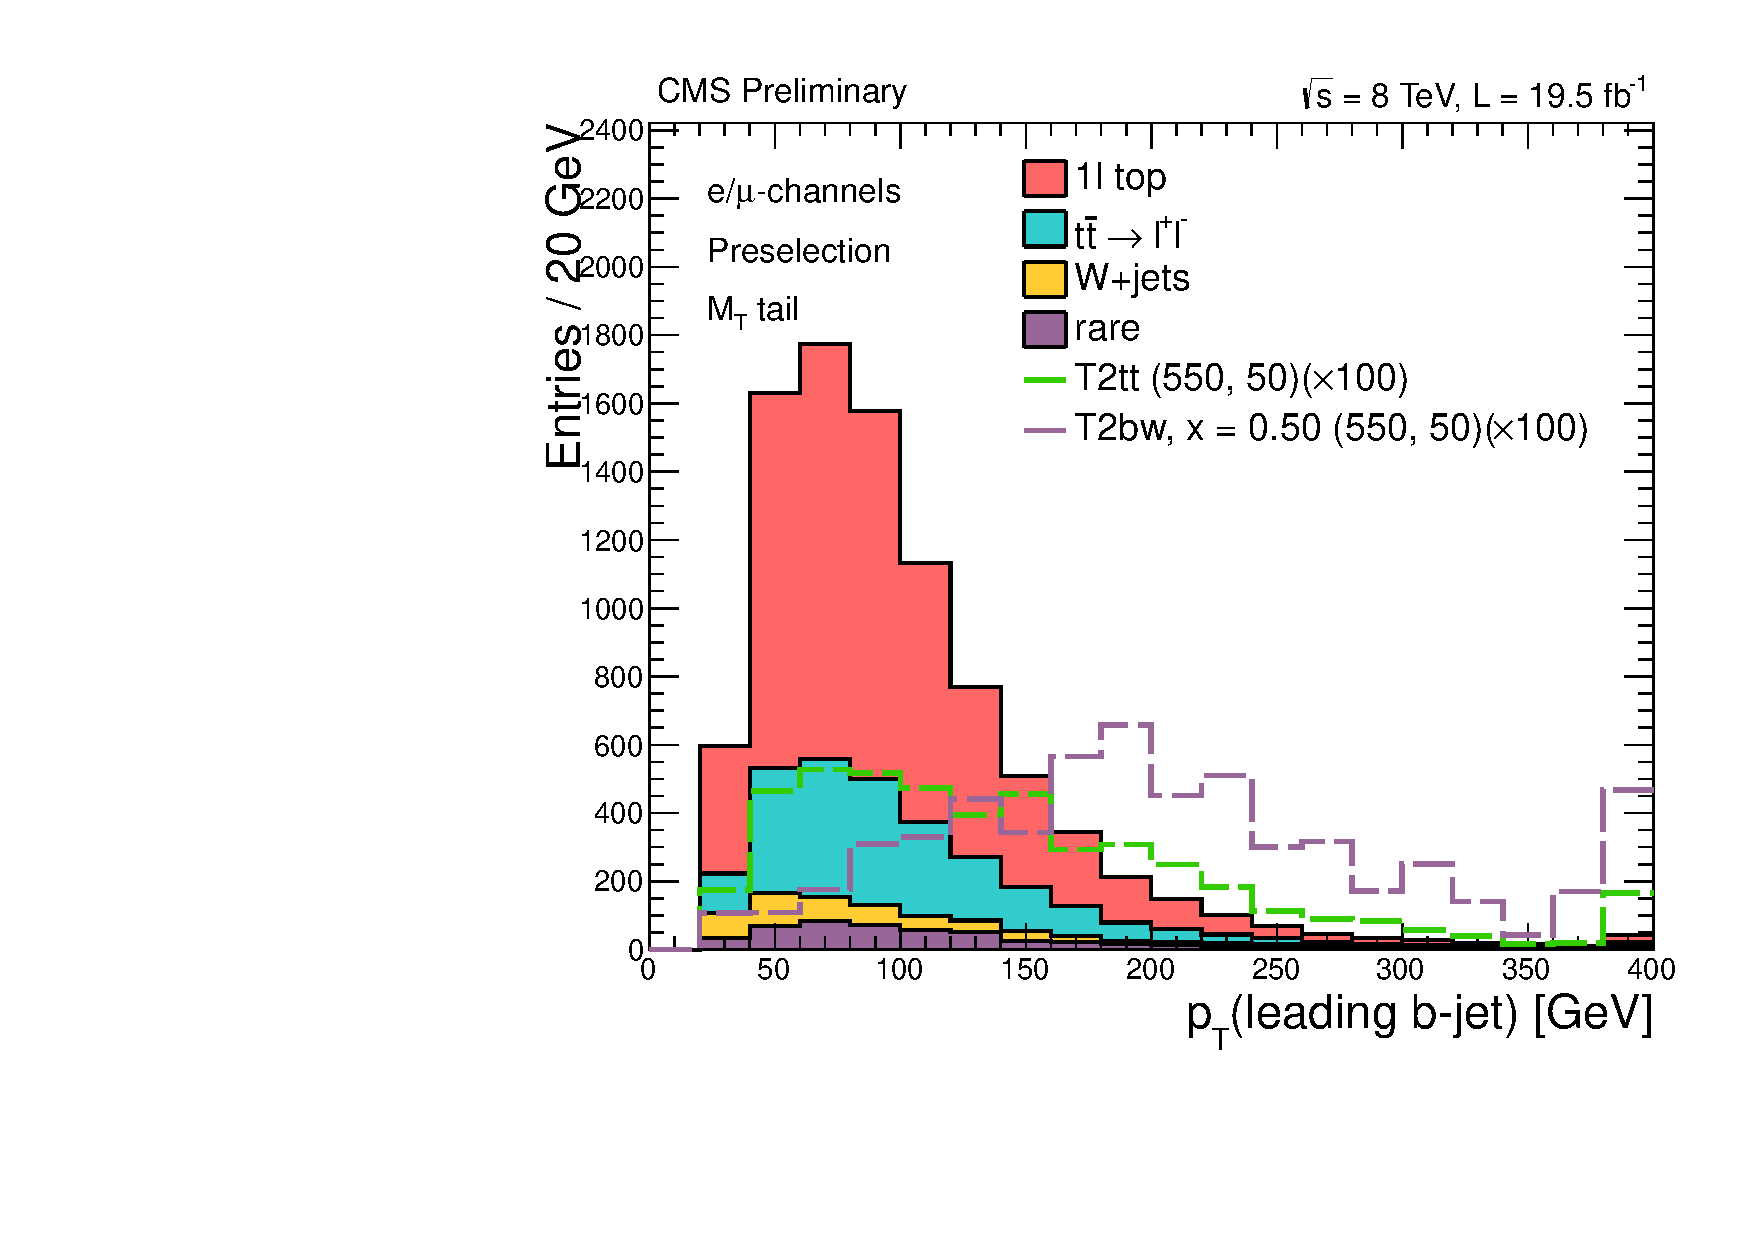
\includegraphics[width=0.32\textwidth]{variables/leadingBPt}
                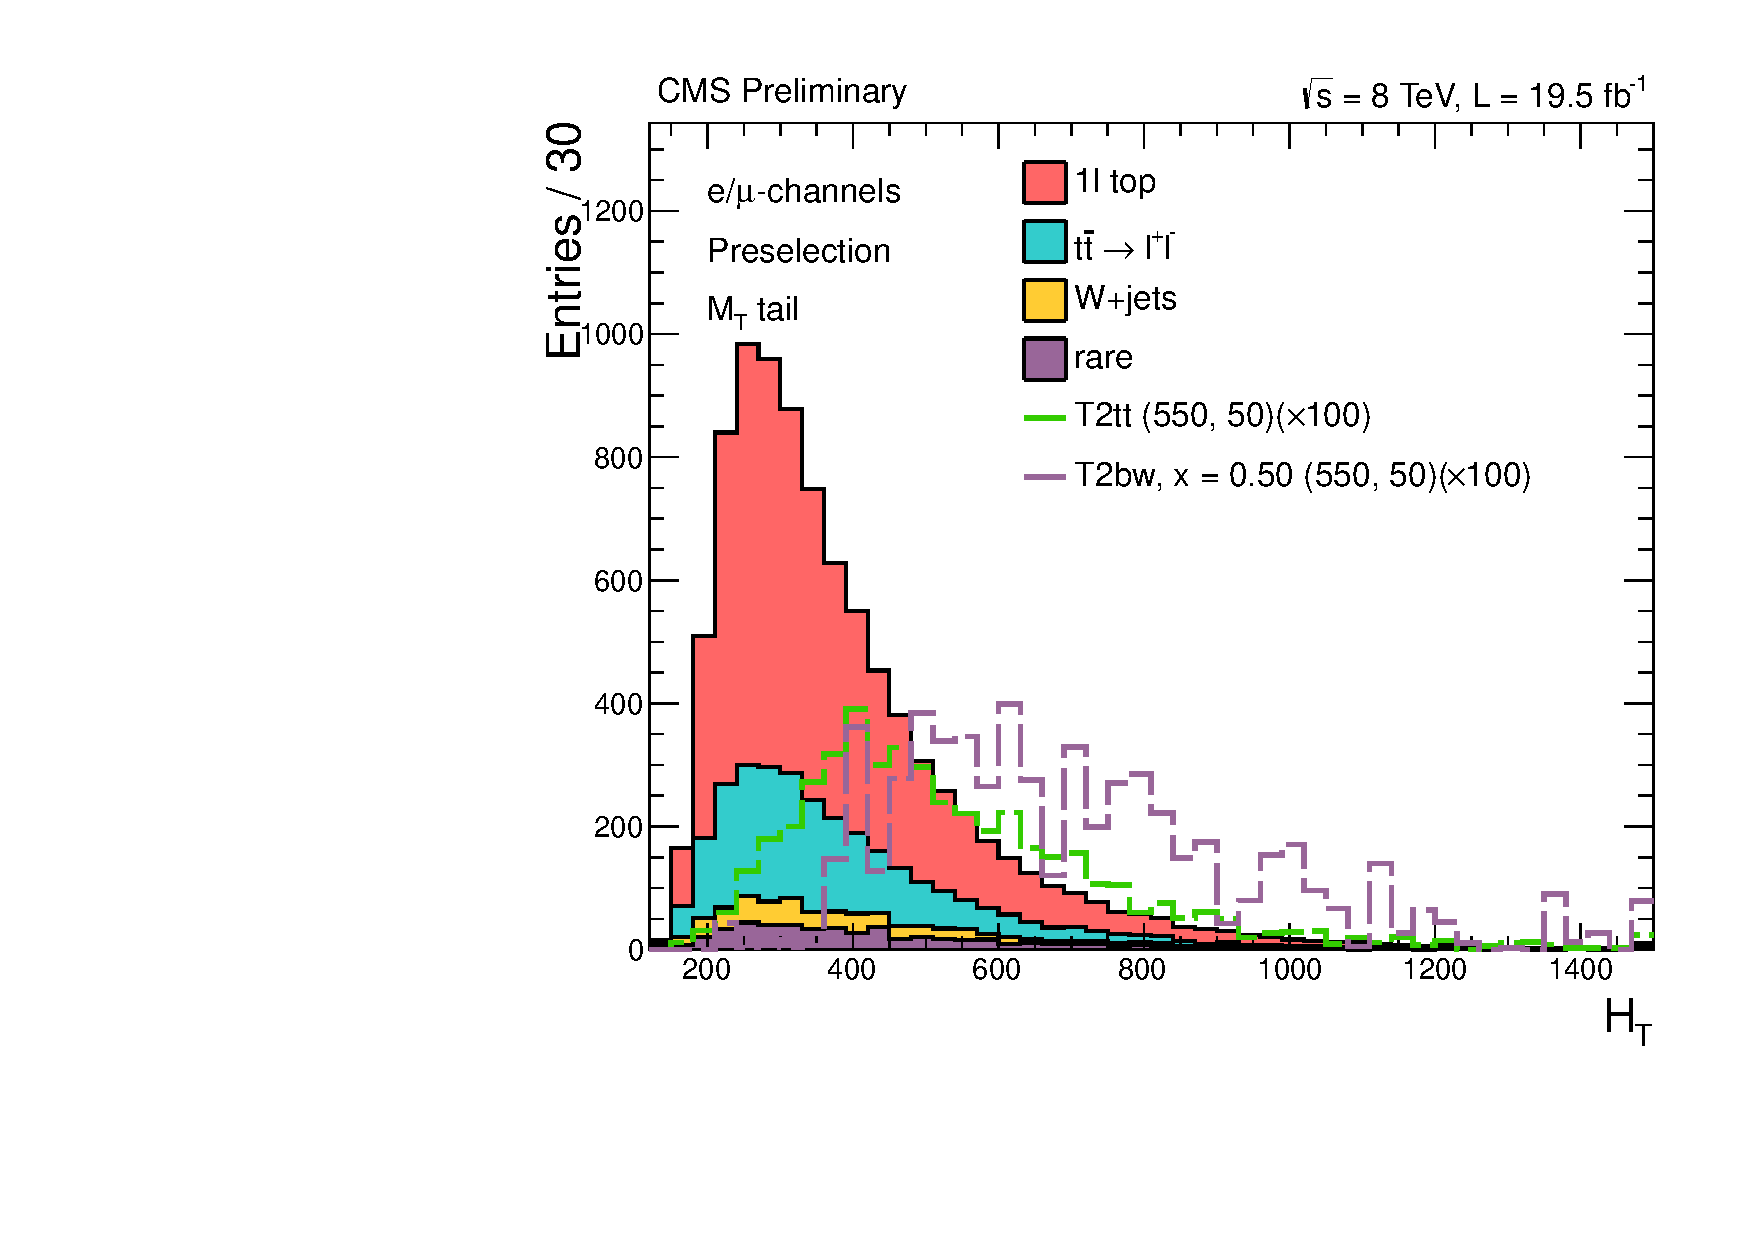
\includegraphics[width=0.32\textwidth]{variables/HT}
                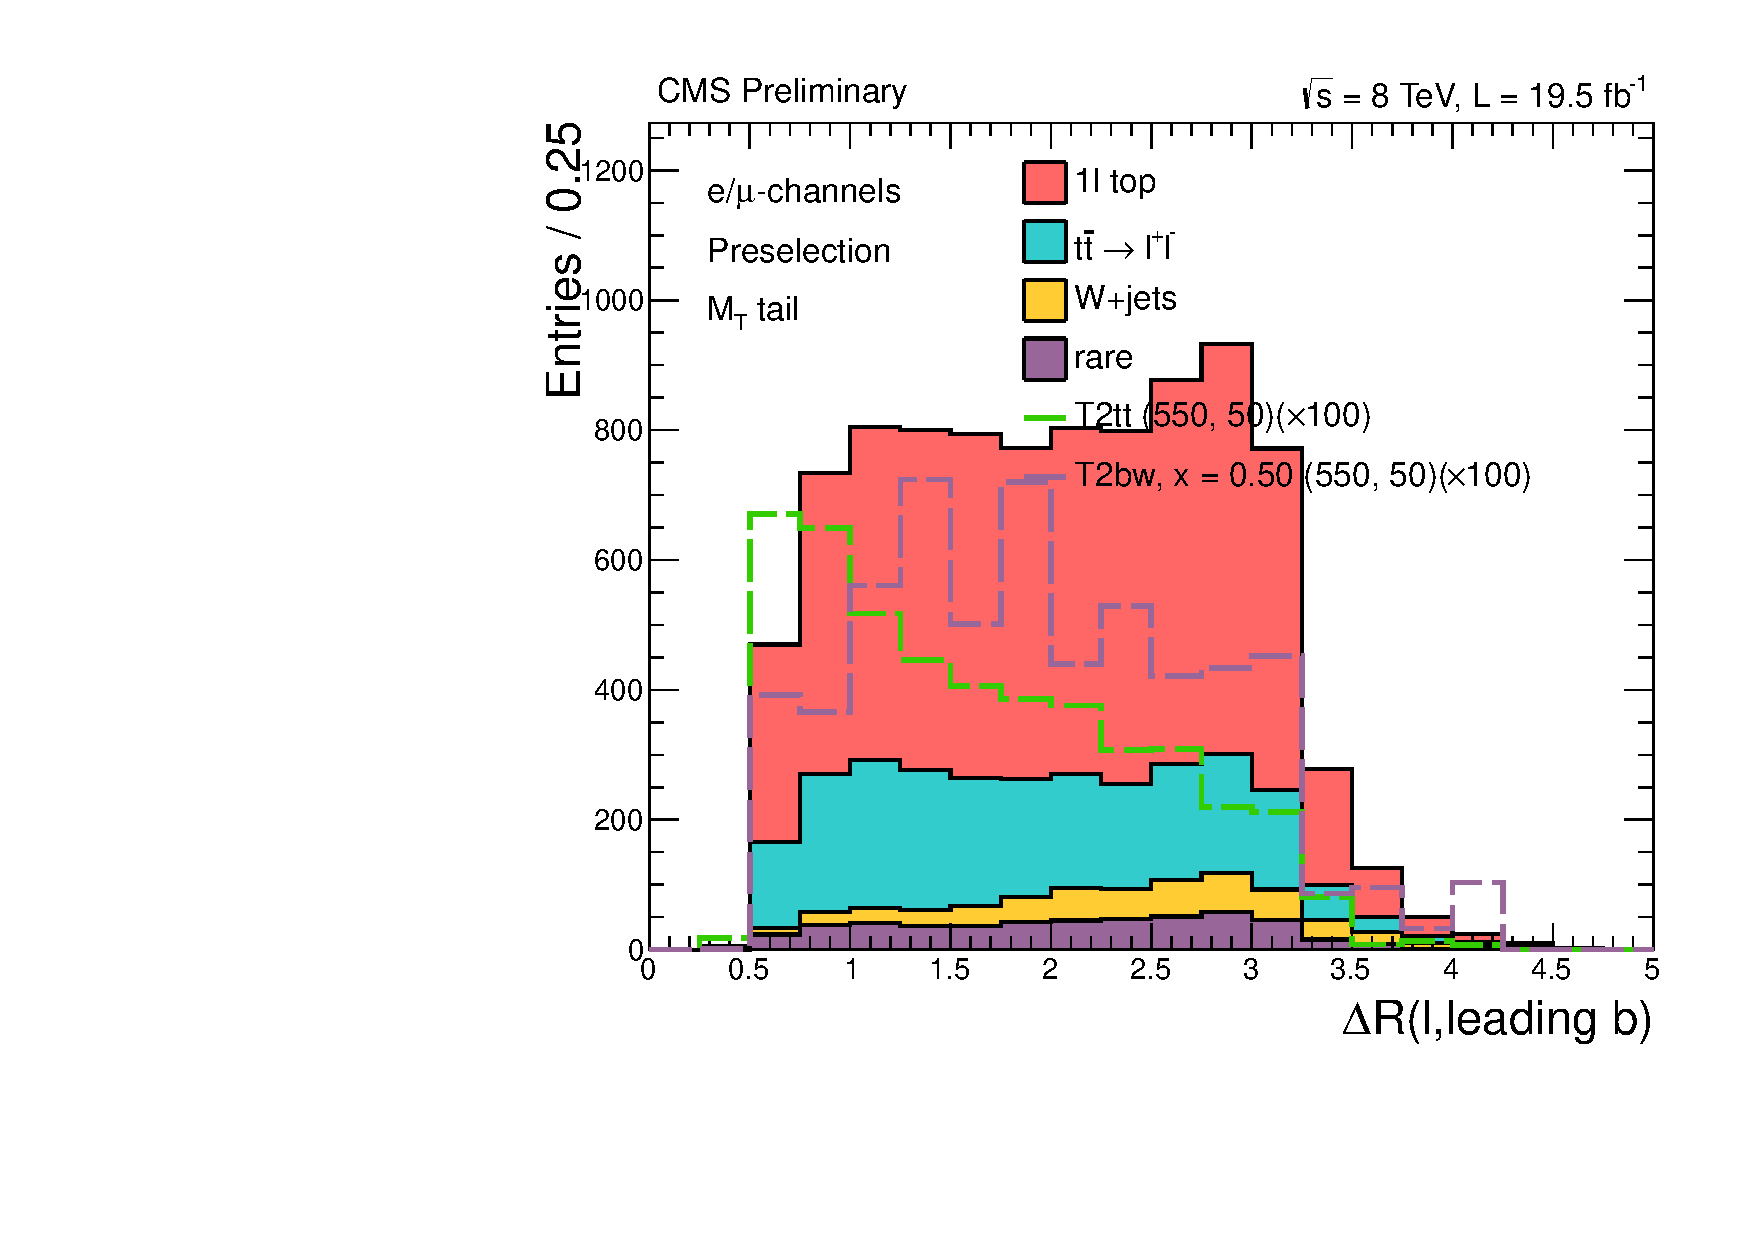
\includegraphics[width=0.32\textwidth]{variables/deltaRLeptonB}\\
                \includegraphics[width=0.32\textwidth]{variables/MET}
                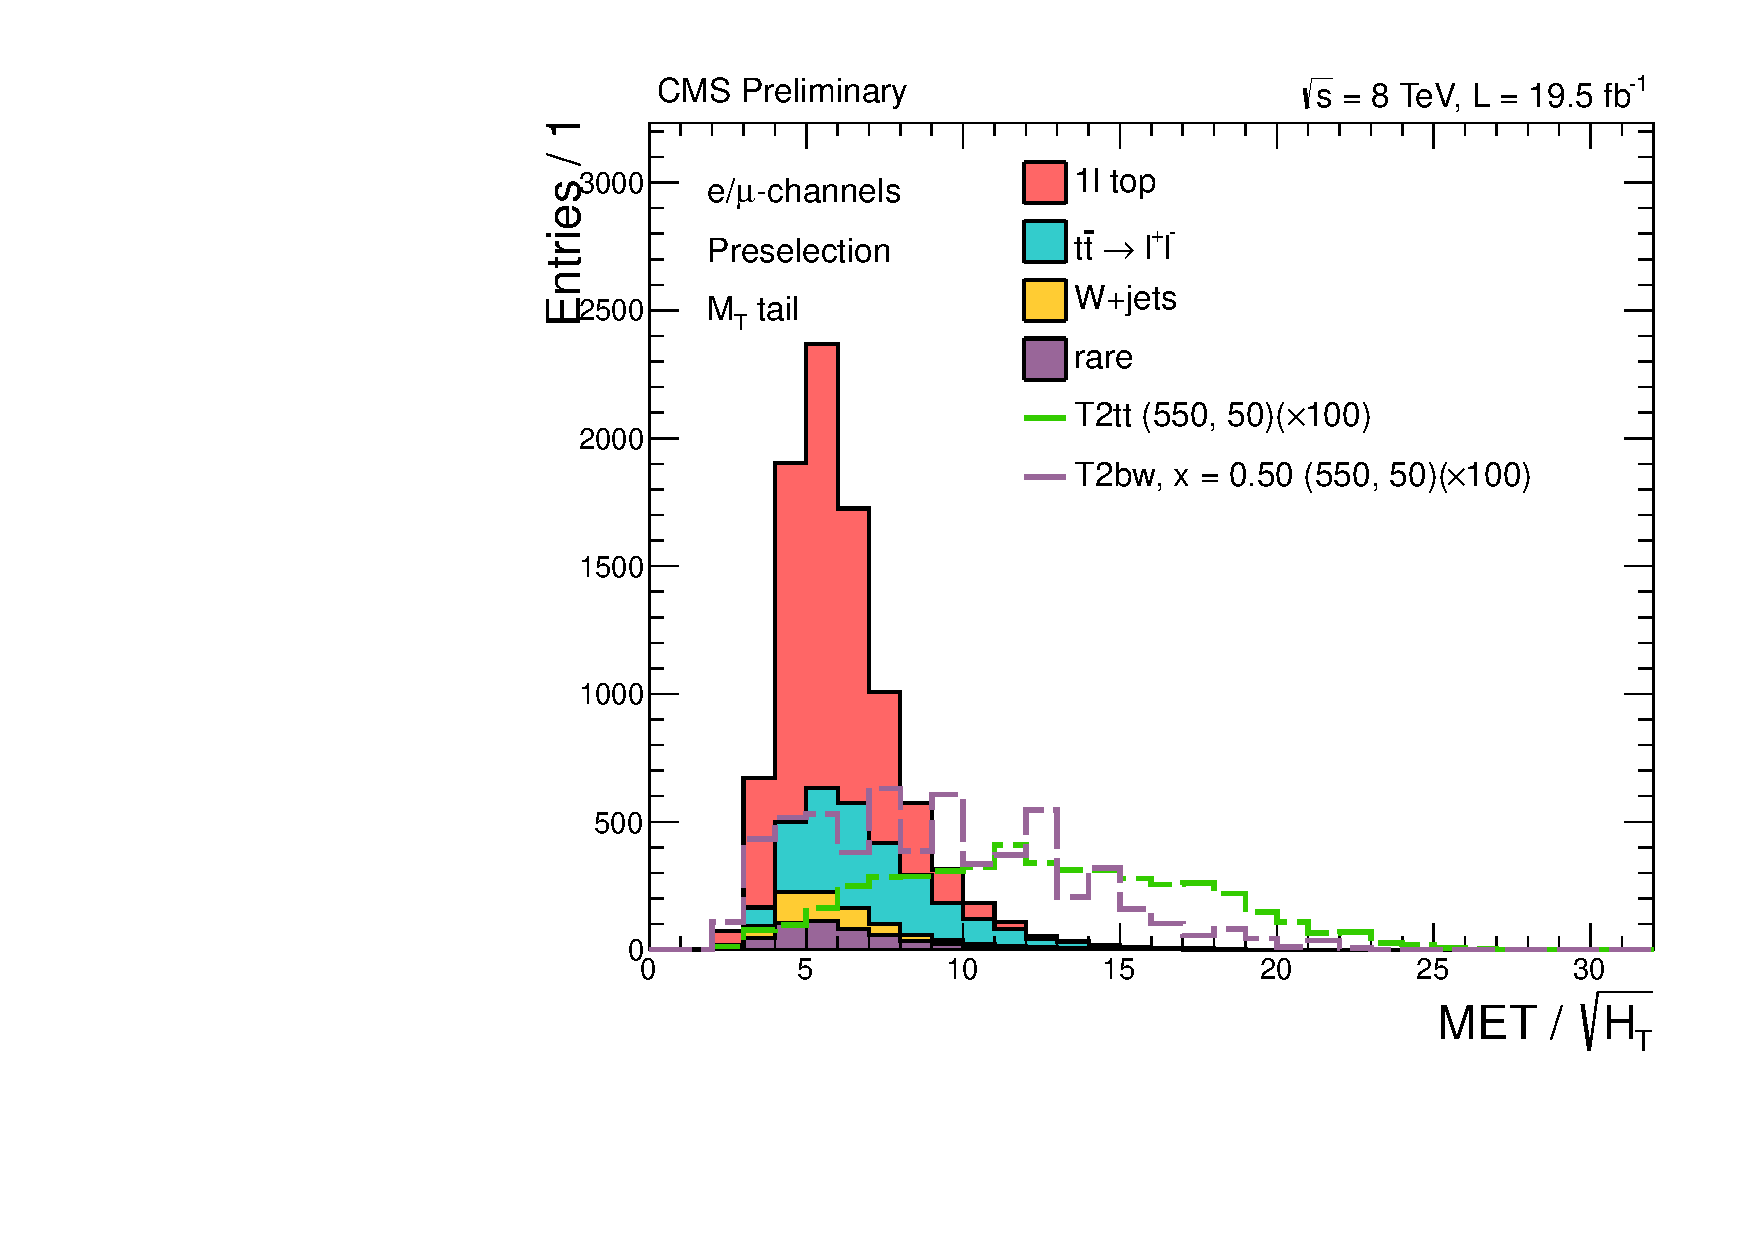
\includegraphics[width=0.32\textwidth]{variables/METoverSqrtHT}
                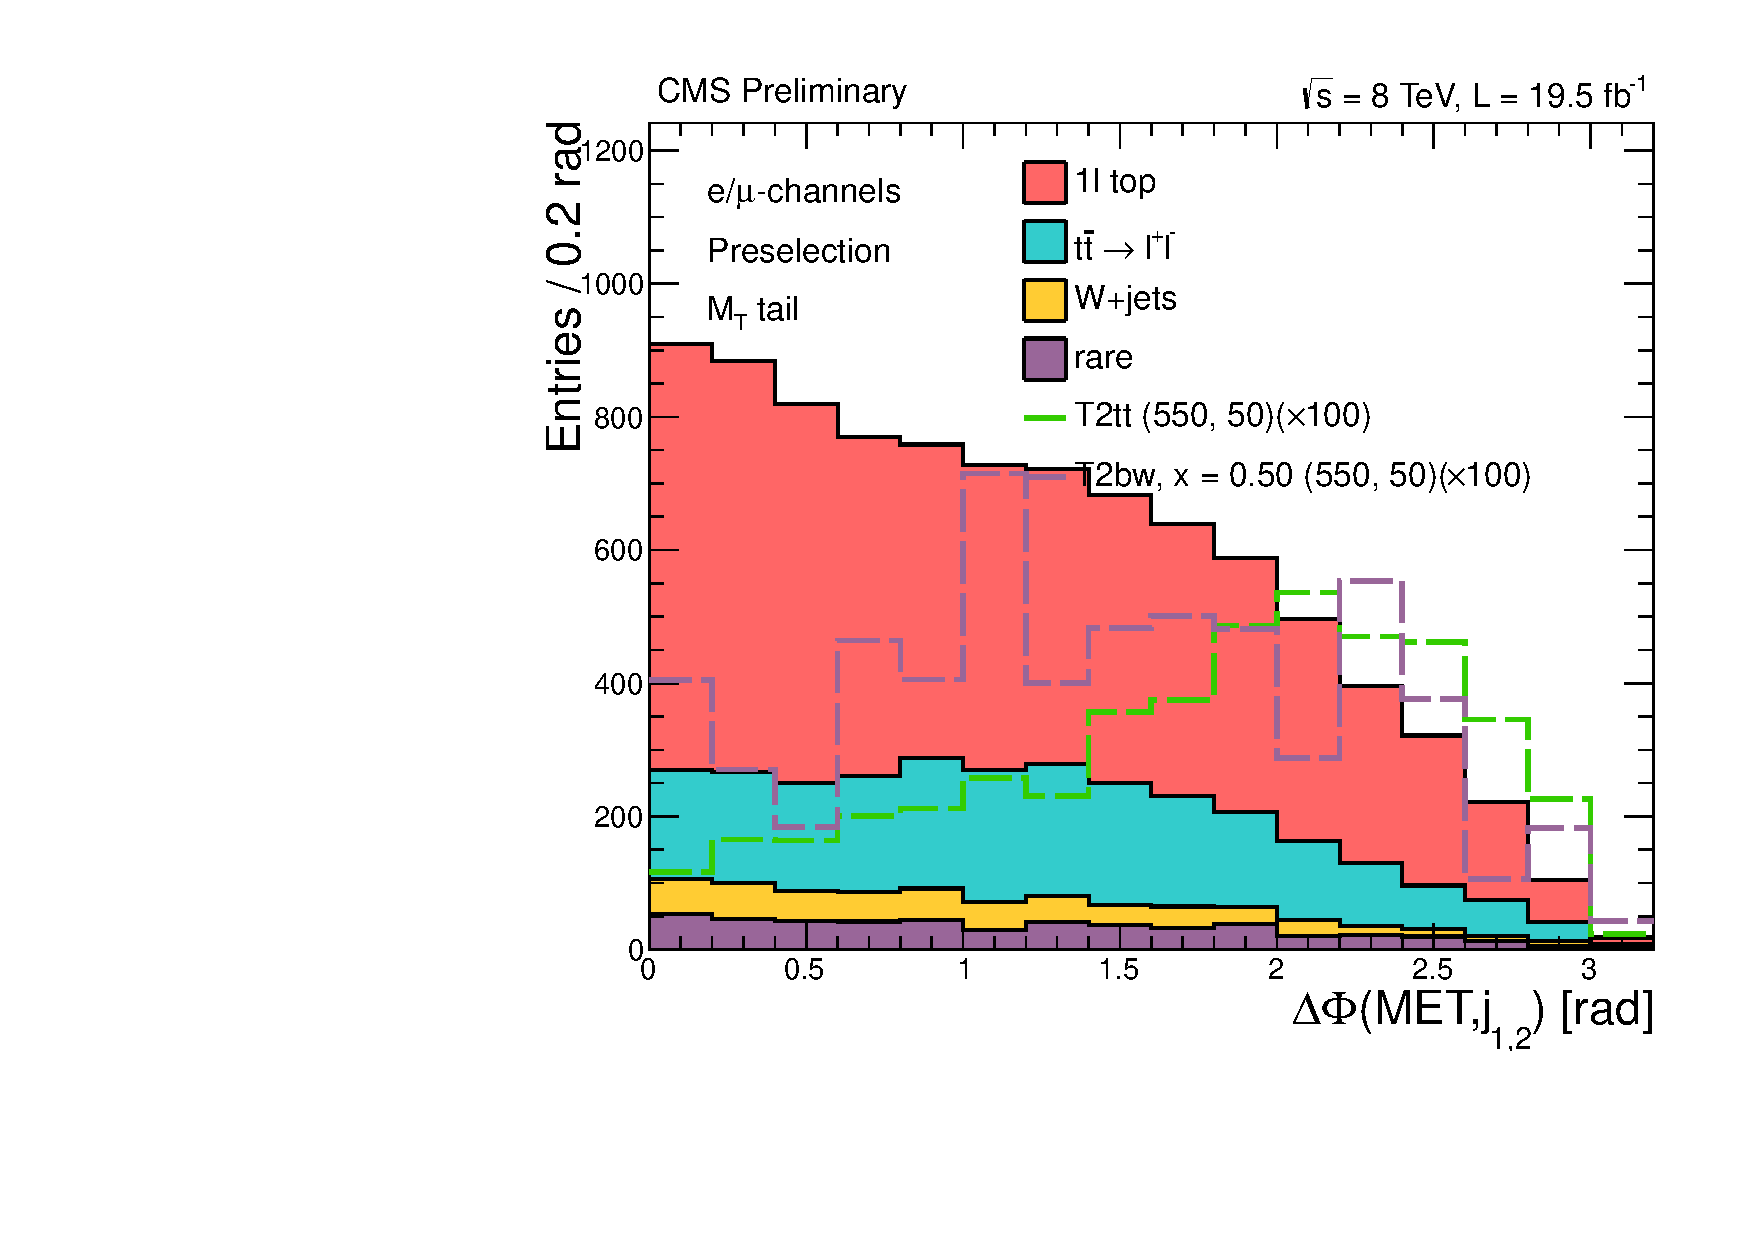
\includegraphics[width=0.32\textwidth]{variables/deltaPhiMETJets}\\
                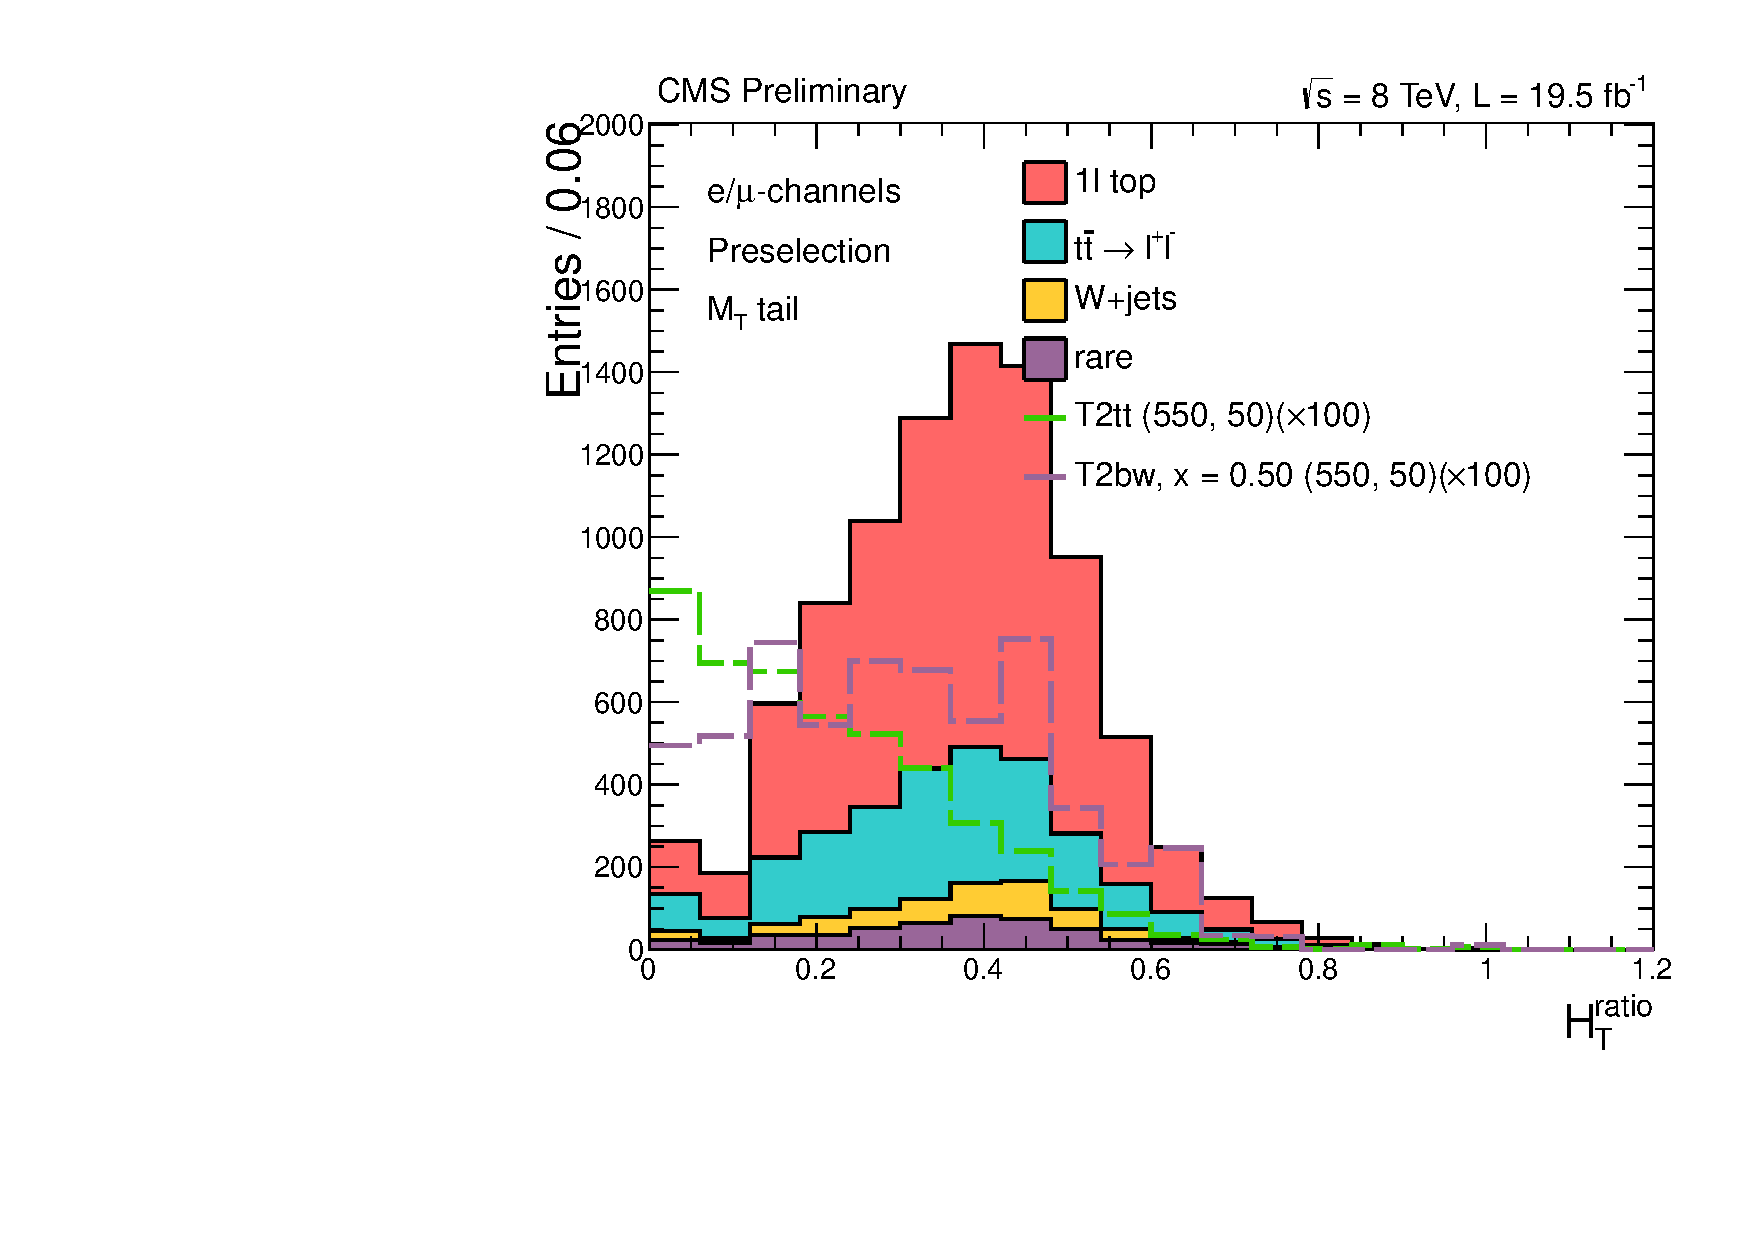
\includegraphics[width=0.32\textwidth]{variables/HTratio}
                \includegraphics[width=0.32\textwidth]{variables/MT2W}
                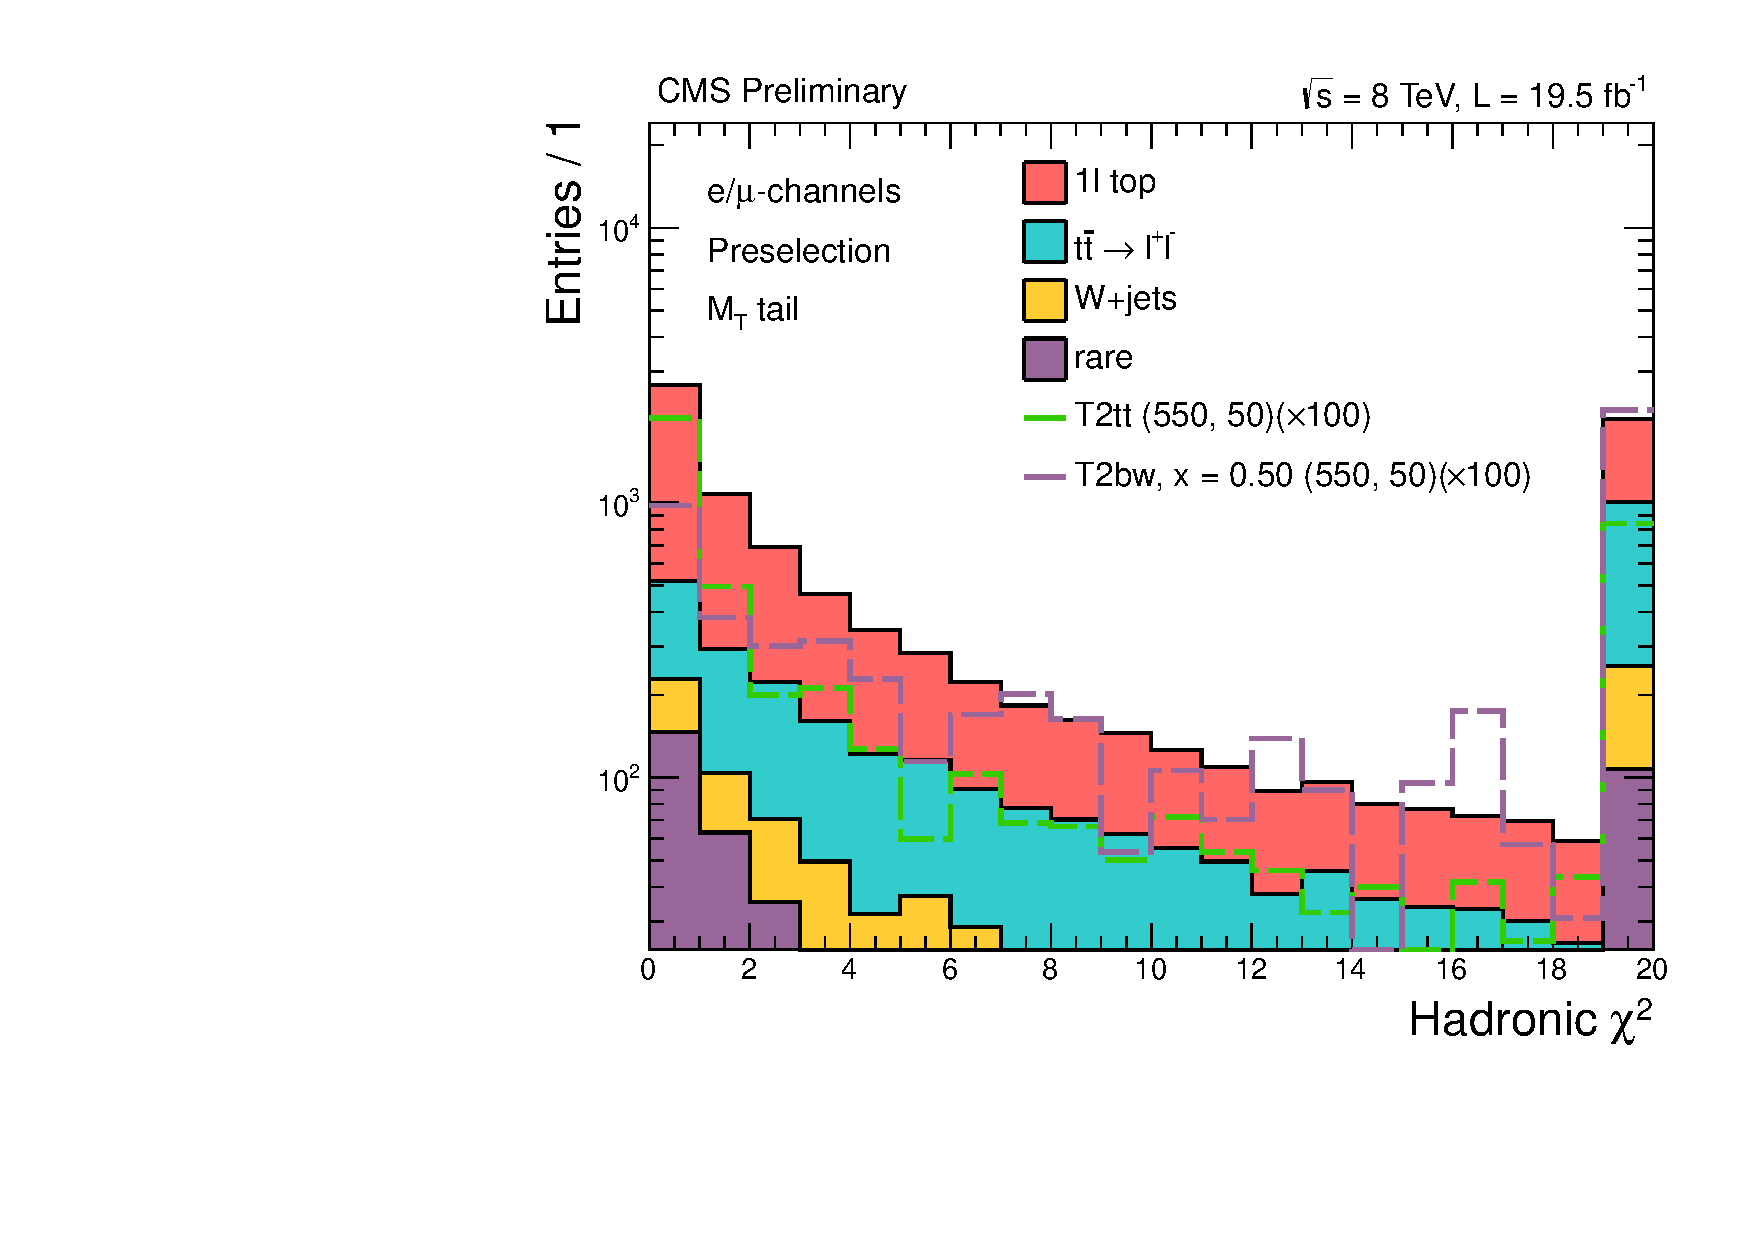
\includegraphics[width=0.32\textwidth]{variables/HadronicChi2}\\
                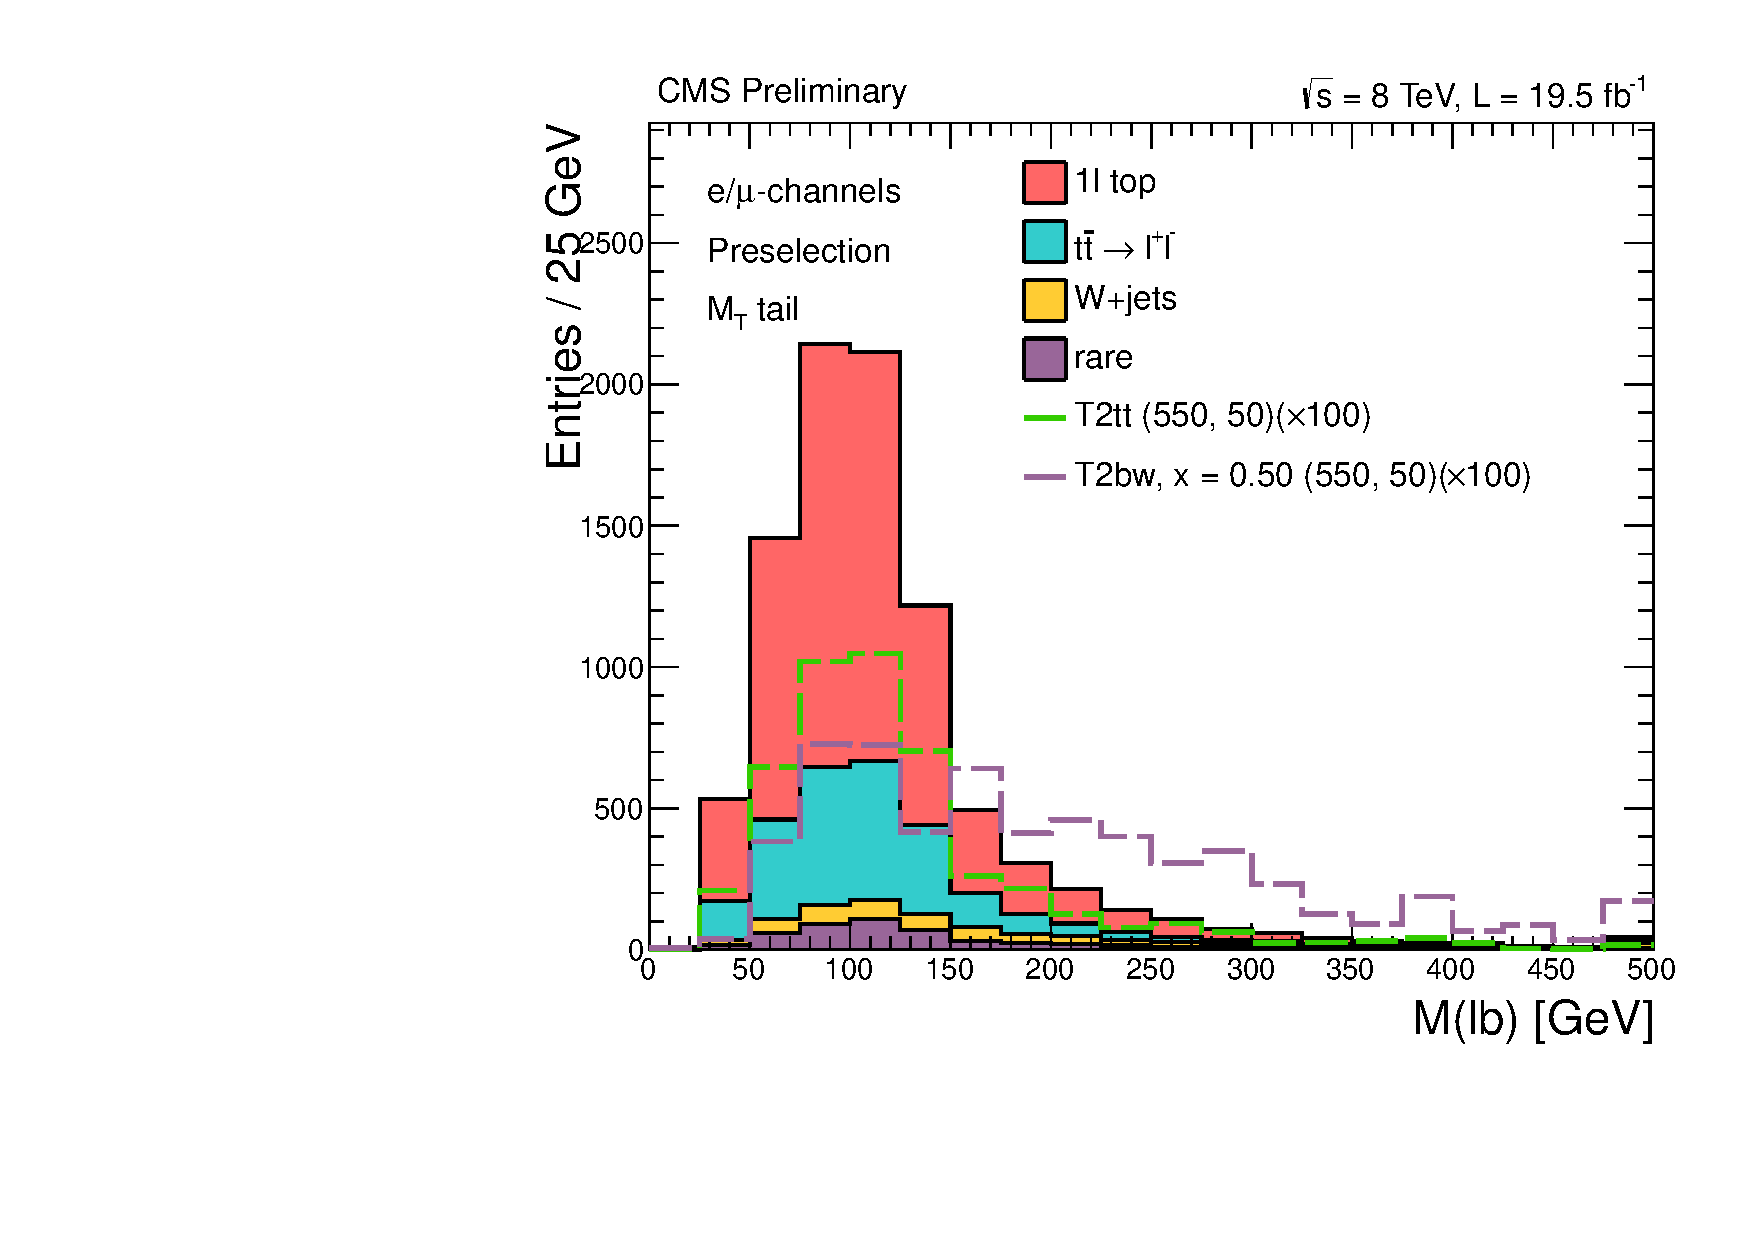
\includegraphics[width=0.32\textwidth]{variables/Mlb_hemi}
                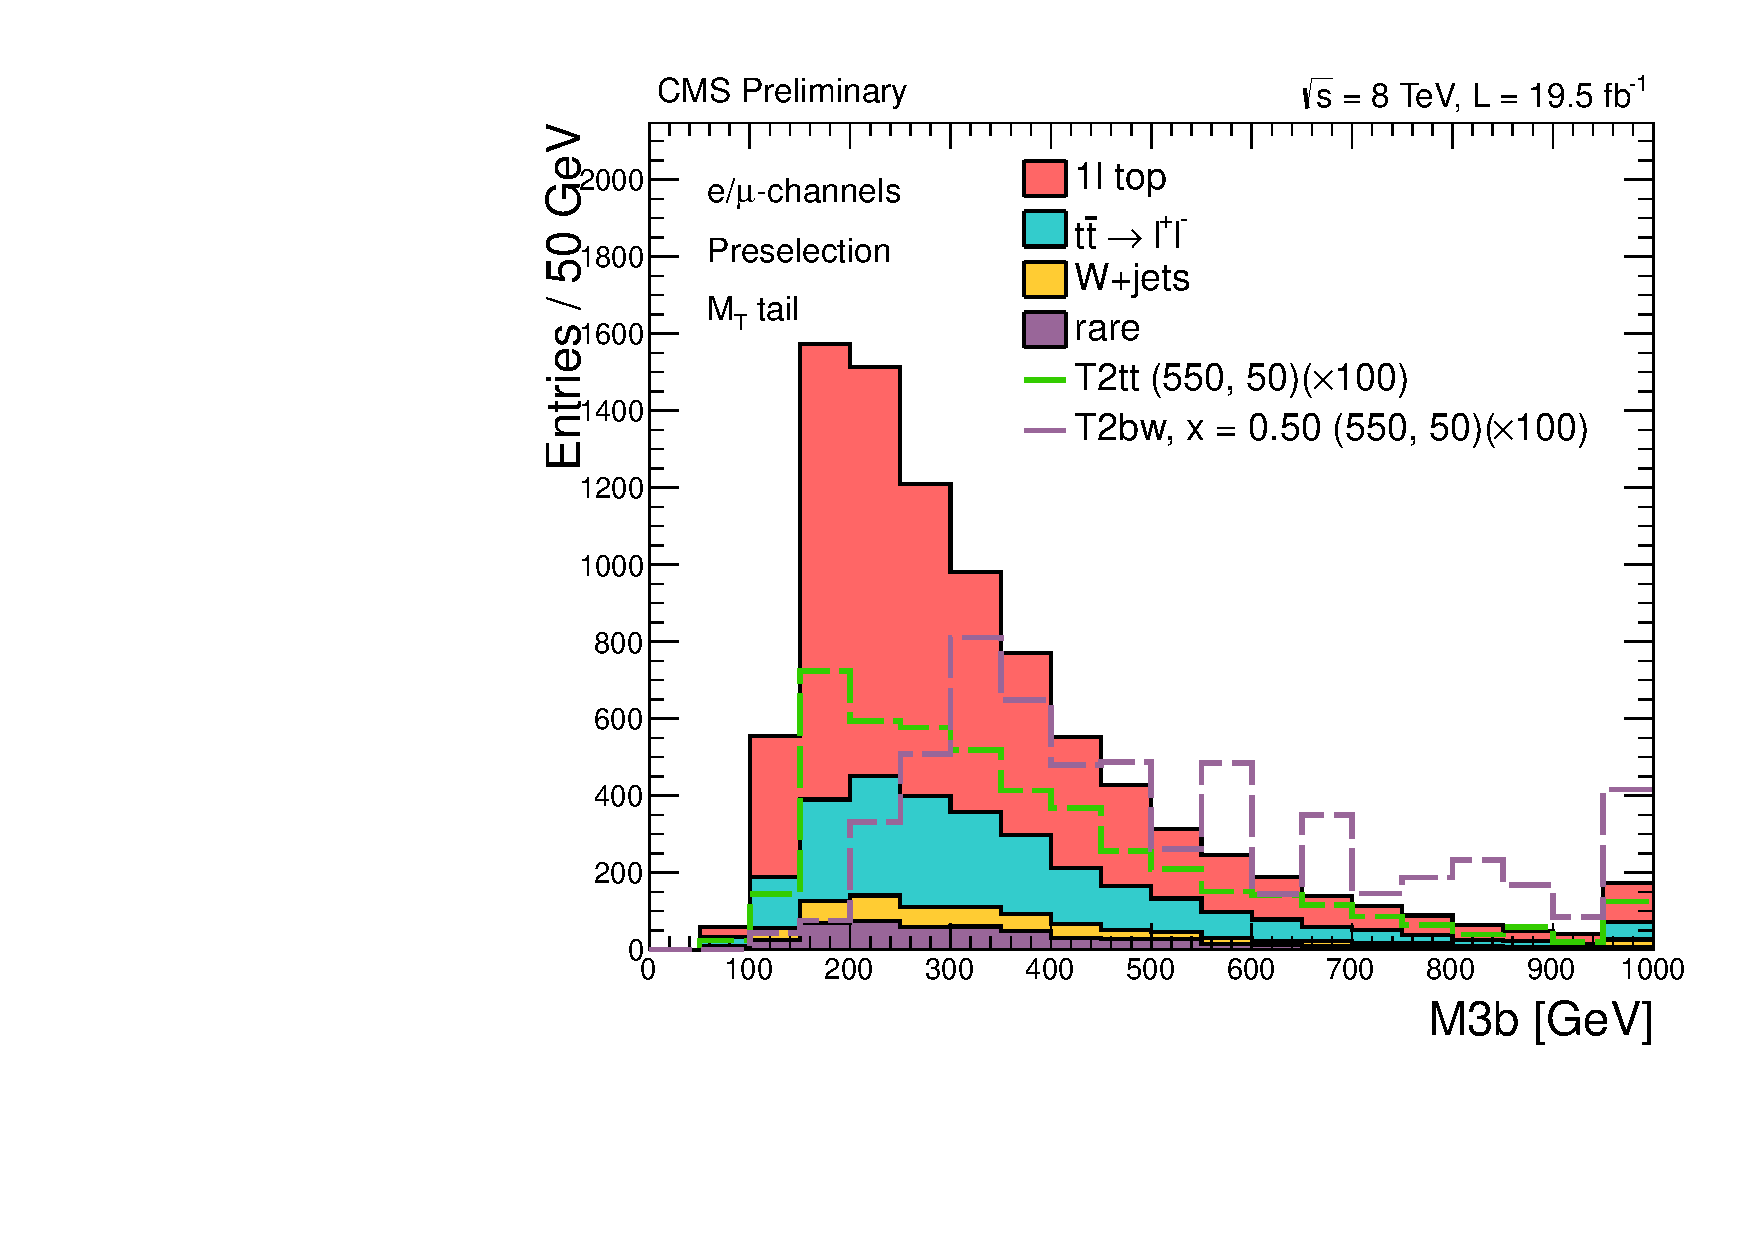
\includegraphics[width=0.32\textwidth]{variables/M3b}
                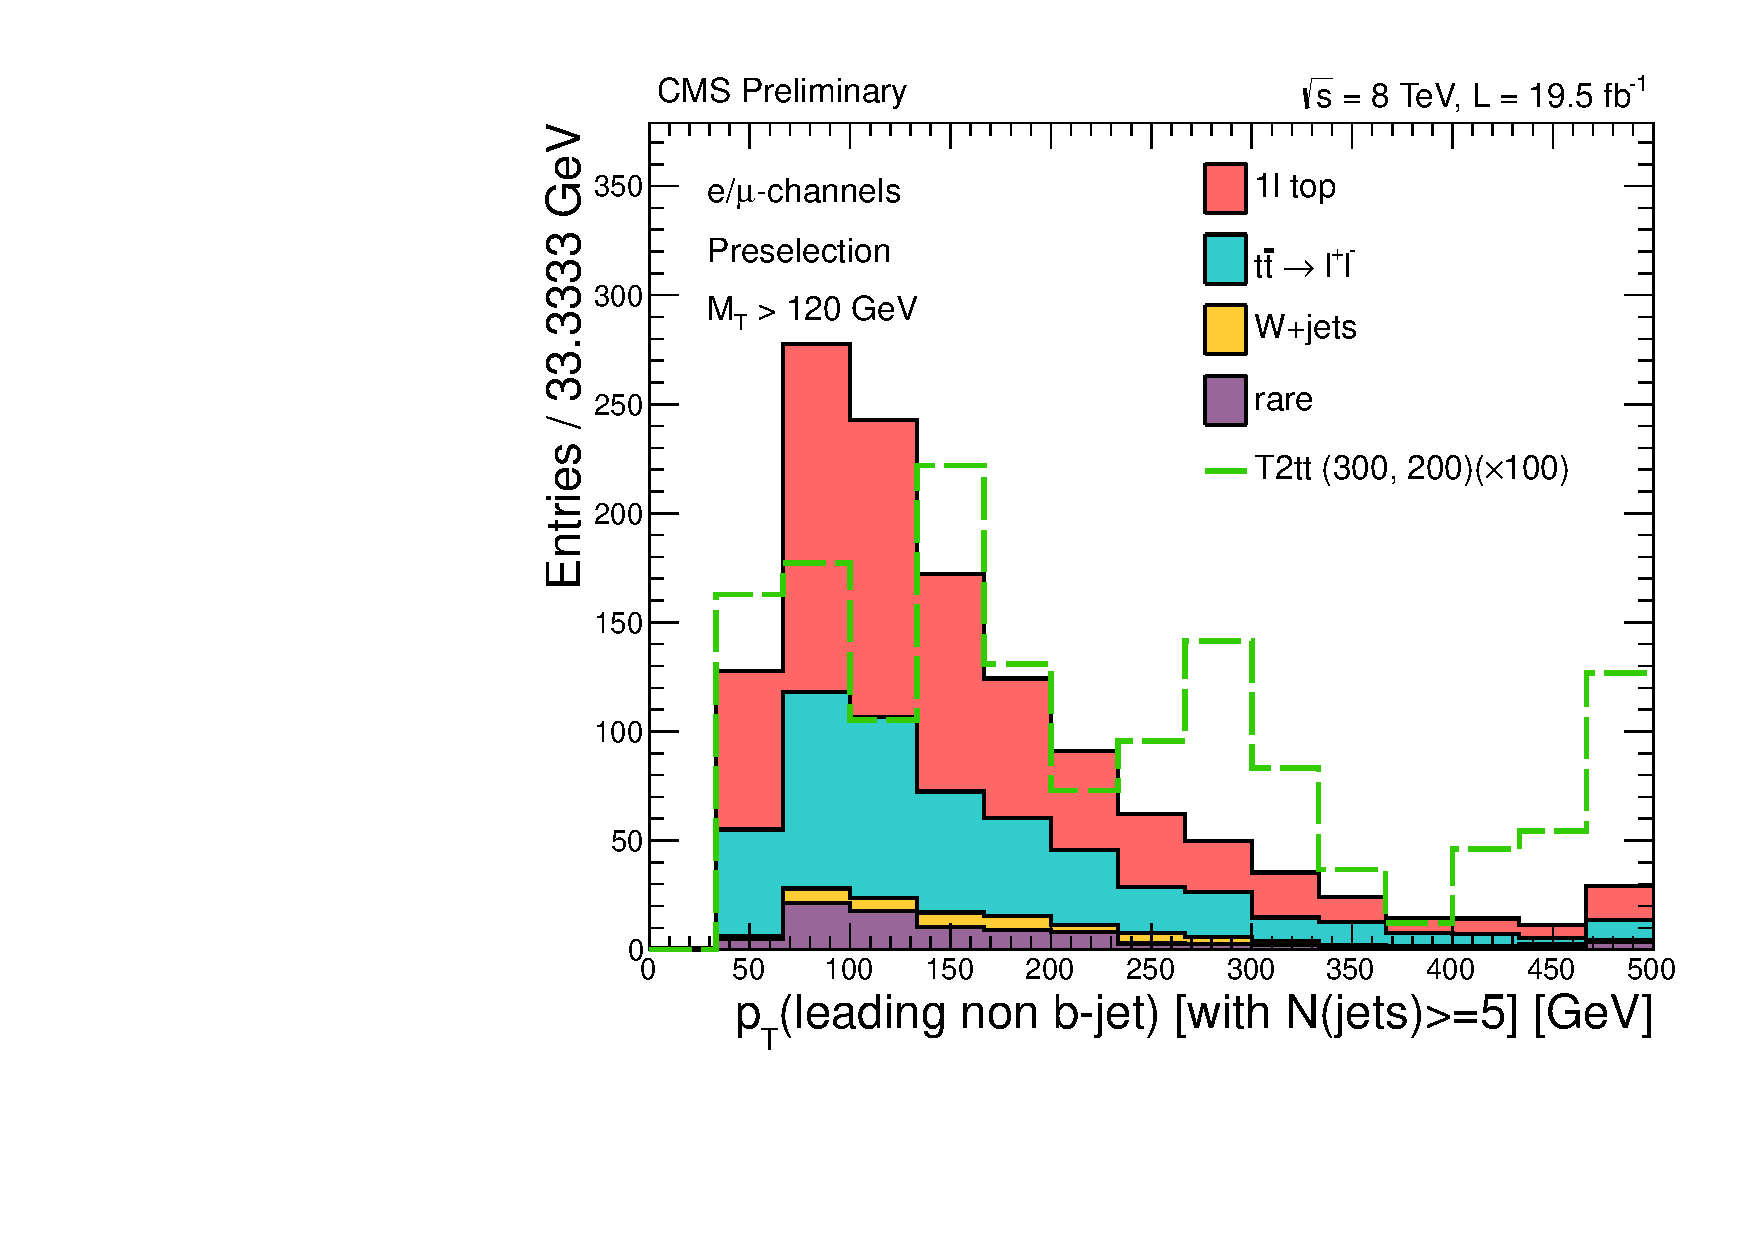
\includegraphics[width=0.32\textwidth]{variables/leadingNonBPtN5}
                \caption{Stacked plots representing the different discriminating variables used to design the signal region, for background and two signal examples after preselection and cut on $M_T > 100 \GeV$.}
                \label{fig:variables}
            \end{figure}

            \subsection{Figure of merit}

            Before going into the details of the signal region optimization, we first need to introduce the
            metric used to do so. The problem of defining cuts to be applied on a variable can be summarized 
            as knowing how to compromise between the quantity of selected signal, $S(\text{cut})$, versus selected
            background, $B(\text{cut})$, such that the sensitivity of the analysis is maximized. Ideally,
            one would run the full statistical interpretation using toy data. However, such a procedure 
            is often CPU intensive and not suitable for an iterative process. A more flexible way is
            to define a figure of merit (FoM) that approximate the statistical interpretation one is aiming
            to perform.

            Let's consider the background only hypothesis $H_0$, also called null hypothesis, and the 
            signal hypothesis $H_1$. These hypothesis are modeled by a probability density function (pdf) of 
            the number of events, as sketched on Figure \ref{fig:interpretation}.
           
            \insertFigure{interpretation}{0.7}
                         {Illustration of the modelization of the hypothesis $H_0$ and $H_1$.}

            From the point of view of excluding a signal, a simple approach consist in computing the type 
            II error (or probability to miss a signal) provided that $D$ events are observed in the
            data. Assuming that the pdf is gaussian, one can express the distance between $D$ and $H_1$ in terms 
            of standard deviations using $(\text{mean}(H_1) - D) / \sigma(H_1) = (S + B - D) / \sqrt{S+B}$.
            The figure of merit can be defined from considering the expected value of this quantity when assuming 
            a toy data equal to $B$, the mean realization of $H_0$ : $\text{FoM}_\text{exclusion} \definedAs S 
            / \sqrt{S+B}$. The same reasonning applies to the point of view of signal discovery, considering 
            the type I error (or probability of false discovery), leading to $\text{FoM}_\text{discovery}
            \definedAs S/\sqrt{B}$.

            The FoM described so far however takes only into account the statistical uncertainty on signal and 
            background but not the systematic aspects. To get a more realistic uncertainty, one can add to 
            $\sigma^2(H)$ a term $f^2 B^2$ where $f$ represents an estimate of the relative systematic uncertainty 
            on the background. Additionally, to work around issues where the remaining statistics becomes low and 
            cuts are not realistic anymore, we ignore cases where $S < 3$ or $B < 1$.

        \subsection{Cut-based signal regions}

            \subsubsection{Optimization procedure}

            The variables are first classified by their individual discriminating power, estimated by taking the 
            maximum FoM achievable on a few signal benchmarks when scanning the possible cuts. The most 
            discriminating variables are $\MT$, $MET$, $MET/\sqrt{H_T}$ and $M_{T2}^{W}$, We also consider 
            $\Delta \phi(j_{1,2},\vec{MET})$, hadronic top $\chi^2$, $p_T(\text{lead. } b)$ and the presence of a
            5th, ISR jet. These variables have low discrimating power at preselection level but get useful after
            additional cuts on $\MT$, $MET$, $MET/\sqrt{H_T}$ and $M_{T2}^W$ depending of the $\deltam$ considered.

            On a few signal benchmarks, we perform a $n$-dimensionnal optimization of the cuts on these variables,
            though not cutting on both $MET$ and $MET/\sqrt{H_T}$ at the same time. During the optimization,
            we include global scale factors on the $\oneLeptonTop$ and $\Wjets$ to mimic the effect of the background
            estimation that will be described later. Typically these categories are considered with a scale factors
            1.3. The otpimisation is done using the exclusion-oriented FoM and assuming a relative systematic uncertainty
            varying between 15 and 30\% depending on the tightness of the cuts. Though we allow tighter cuts on $\MT$
            than the starting point $> 120 \GeV$, the cut is constrained to not be higher than $> 140 \GeV$ to keep
            enought statistics for the background estimation.

            After optimizing on a few benchmarks, a set of list of cuts is defined and a systematic check accross the
            $(\mass{\lstop},\mass{\lneutralino})$ plane is performed to keep the most performing list of cuts. For the
            sake of simplicity, we then proceed to a manual clustering of similar lists and remove cuts that do not 
            significantly improve the performances.

            \subsubsection{Results and performances}

            The resulting list of cuts are presented on Table \ref{tab:cutAndCountCuts} and Figure \ref{fig:cutAndCountPerformances}
            shows the best performing set accross the $(\mass{\lstop},\mass{\lneutralino})$ plane as well as the
            corresponding FoM.

            \begin{table}[!ht]
                {\footnotesize
            \begin{center}
            \hspace*{-0.8cm}
                    \begin{tabular}{|l|ccccccc|}
                        \hline
                        \textbf{T2tt}          & $\MT$   & $MET$    & $MET/\sqrt{H_T}$  & $M_{T2}^W$ & Hadronic top $\chi^2$ & $\Delta\phi(j_{1,2},\vec{MET})$      &   5th, ISR jet \\
                    \hline                                                                                                                                     
                    1) off-shell (loose)       & $>$ 125 & -       &   $>$ 8            &     -     & -             &          - &    yes        \\
                    2) off-shell (tight)       & $>$ 130 & $>$ 300 &   -                &     -     & -        	    &          - &    yes        \\
                    3) low    $\mass{\lstop}$  & $>$ 140 & -       &   $>$ 8            &     -     &  $<$ 5        &  $>$ 0.8   &    -          \\
                    4) medium $\deltam$        & $>$ 140 & $>$ 200 &   -                &  $>$ 180  &  $<$ 3        &  $>$ 0.8   &    -          \\
                    5) high   $\deltam$        & $>$ 130 & $>$ 350 &   -                &  $>$ 190  & -             &          - &    -          \\
                        \hline
                    \end{tabular}
            \hspace*{-0.5cm}
                    \begin{tabular}{|l|ccccccc|}
                        \hline
                        \textbf{T2bw}, $x$ = 0.25        & $\MT$     & $MET$    & $MET/\sqrt{H_T}$ & $M_{T2}^W$ & $\pT(\text{lead. }b)$ & $\Delta\phi(j_{1,2},\vec{MET})$ & 5th, ISR jet  \\
                    \hline                                                                                                                      
                    1) off-shell       & $>$ 120   &  -       &    $>$  9       &     -      &   -                   &  $>$ 0.2      & yes           \\
                    2) low    $\deltam$ & $>$ 120   &  -       &    $>$  6       &  $>$ 200   & $>$ 180               &  $>$ 0.8      & -             \\
                    3) high   $\deltam$ & $>$ 120   & $>$ 300  &     -           &  $>$ 200   & $>$ 180               &  $>$ 0.8      & -             \\
                    \hline
                      \textbf{T2bw}, $x$ = 0.50       & $\MT$     & $MET$    & $MET/\sqrt{H_T}$ & $M_{T2}^W$ & $\pT(\text{lead. }b)$ & $\Delta\phi(j_{1,2},\vec{MET})$ & 5th, ISR jet  \\
                        \hline
                    1) off-shell       &  $>$ 120  &   -      &  $>$  9         &    -       & -                     &  $>$ 0.2      & yes           \\
                    2) low masses      &  $>$ 135  &   -      &  $>$  6         & $>$ 180    & -                     &  $>$ 0.8      & -             \\
                    3) medium $\deltam$ &  $>$ 140  &   -      &  $>$  7         & $>$ 190    & $>$ 100               &  $>$ 0.8      & -             \\
                    4) high   $\deltam$ &  $>$ 120  & $>$ 300  &   -             & $>$ 200    & $>$ 100               &  $>$ 0.8      & -             \\
                        \hline
                        \textbf{T2bw}, $x$ = 0.75     & $\MT$     & $MET$    & $MET/\sqrt{H_T}$ & $M_{T2}^W$ & $\pT(\text{lead. }b)$ & $\Delta\phi(j_{1,2},\vec{MET})$ & 5th, ISR jet  \\
                        \hline
                    1) low    $\deltam$ &  $>$ 120  &   -      &  $>$  12        &     -      &      -                &  $>$ 0.8      & yes           \\
                    2) medium $\deltam$ &  $>$ 130  &   -      &  $>$  10        &  $>$ 180   &      -                &  $>$ 0.8      & -             \\
                    3) high   $\deltam$ &  $>$ 140  & $>$ 300  &    -            &  $>$ 200   &      -                &  $>$ 0.8      & -             \\
                        \hline                                                 
                    \end{tabular}
            \caption{Description of the ten different signal regions defined for T2bw. \label{tab:cutAndCountCuts}} 
            \end{center}}
            \end{table}


            \begin{figure}[h!]
                \centering
                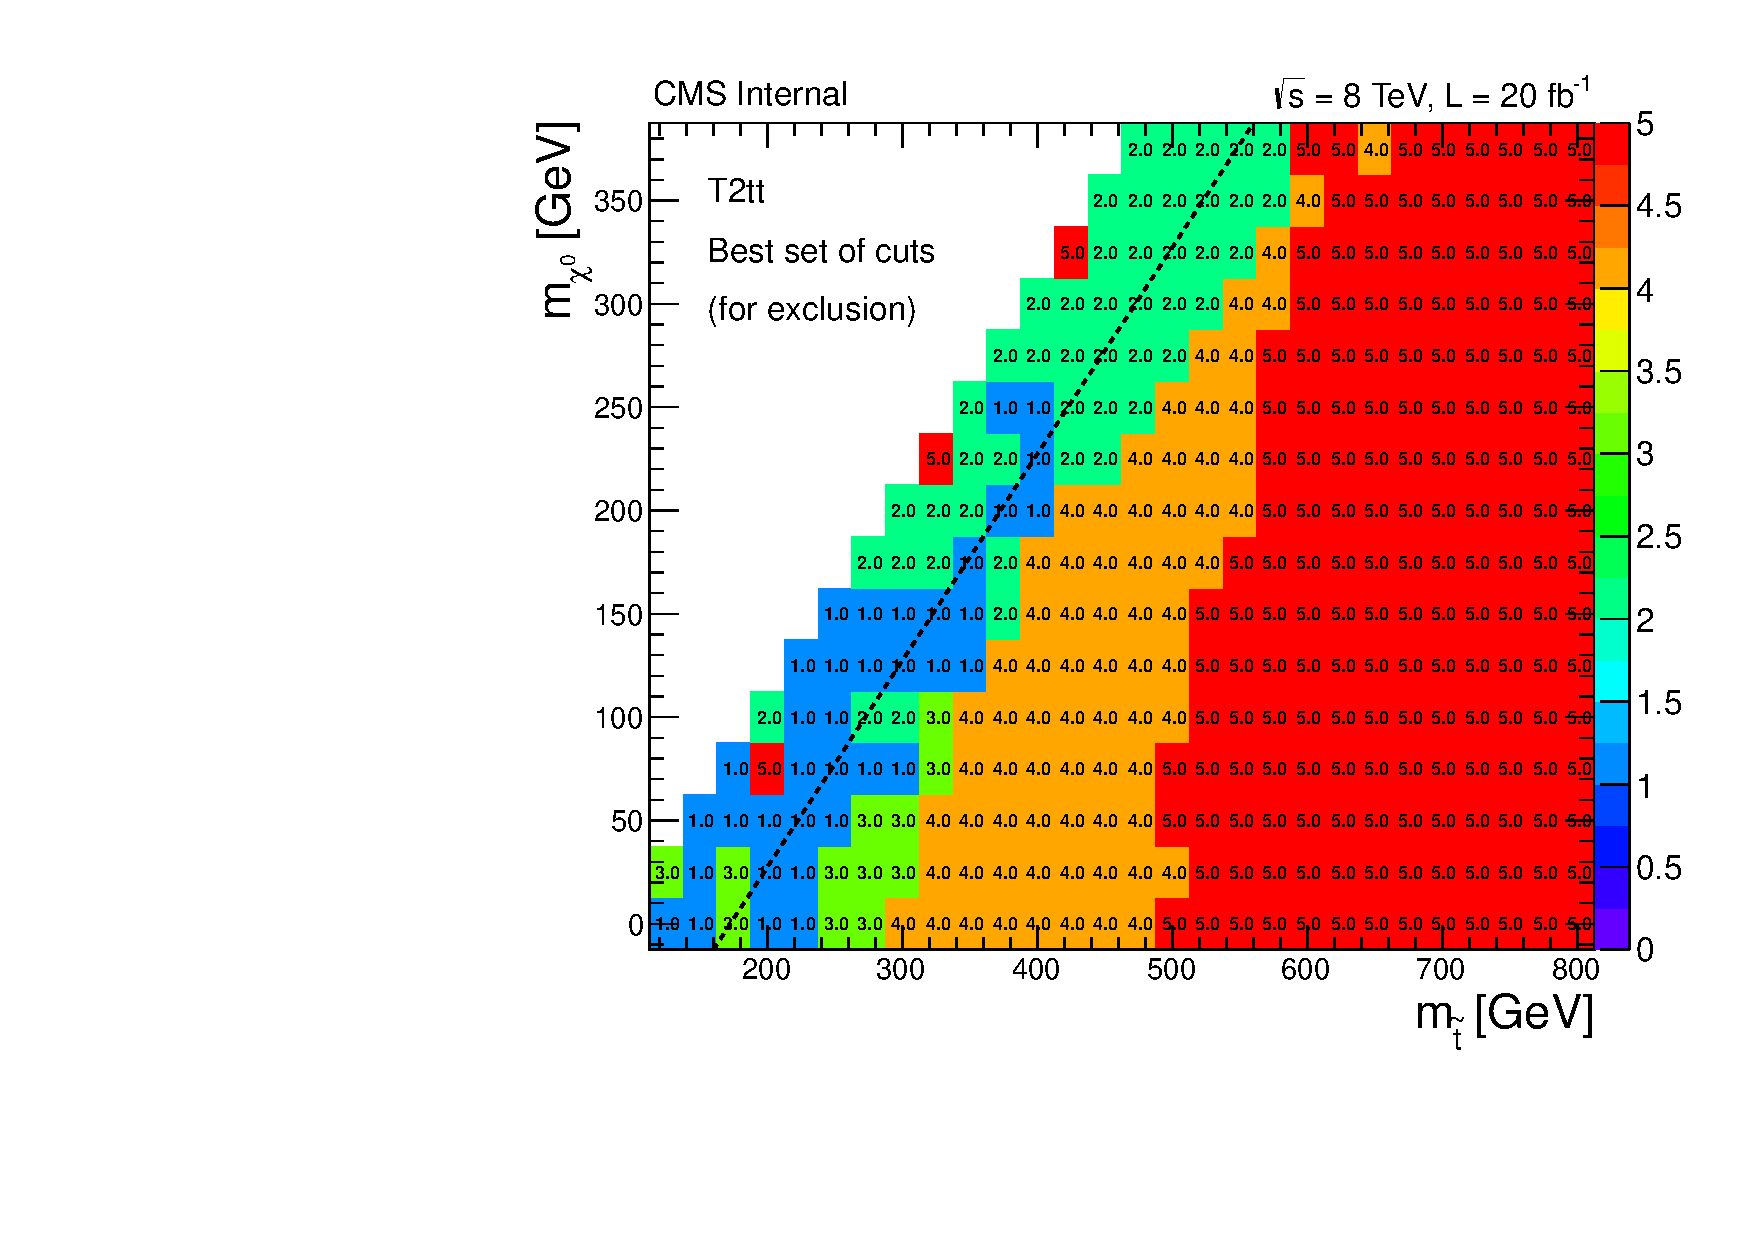
\includegraphics[width=0.36\textwidth]{cutAndCountPerformances/bestSet_T2tt}
                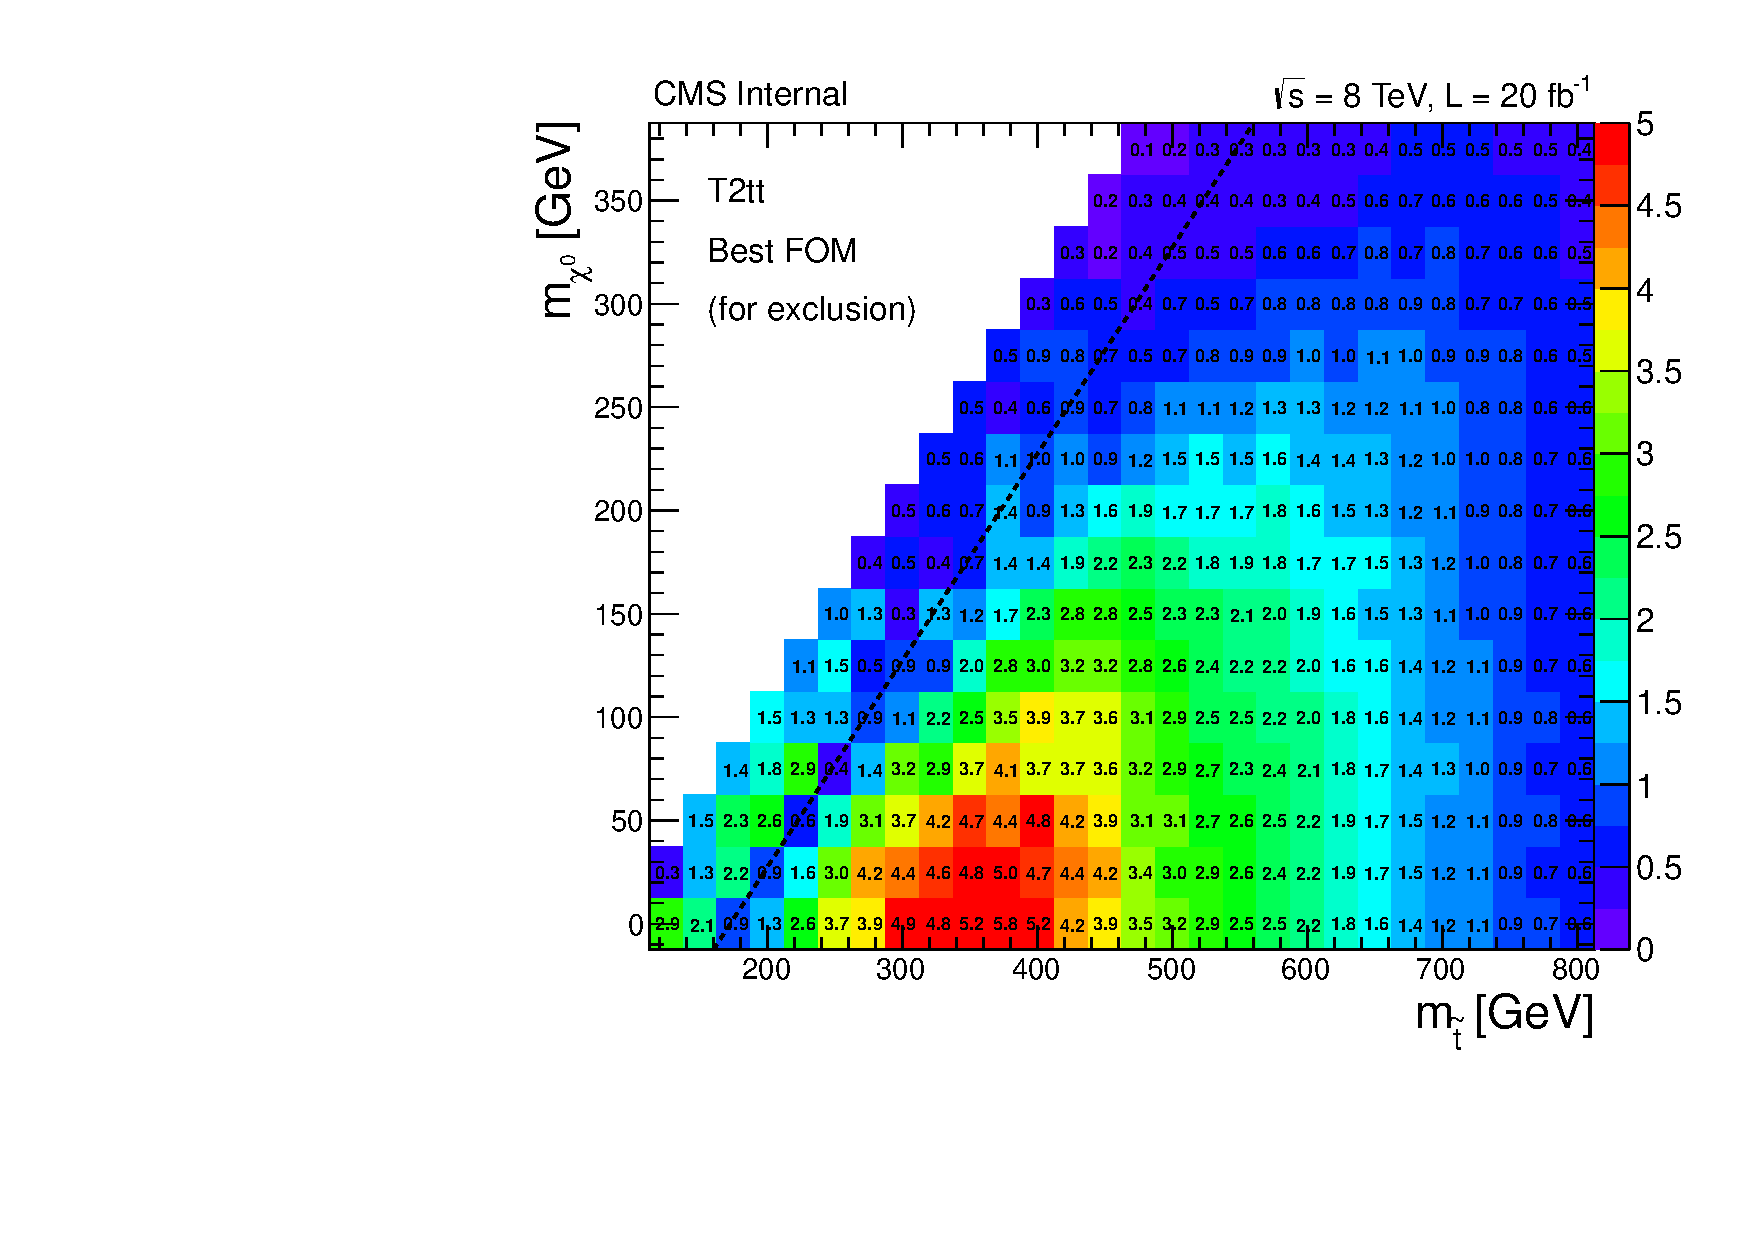
\includegraphics[width=0.36\textwidth]{cutAndCountPerformances/bestFOM_T2tt}\\
                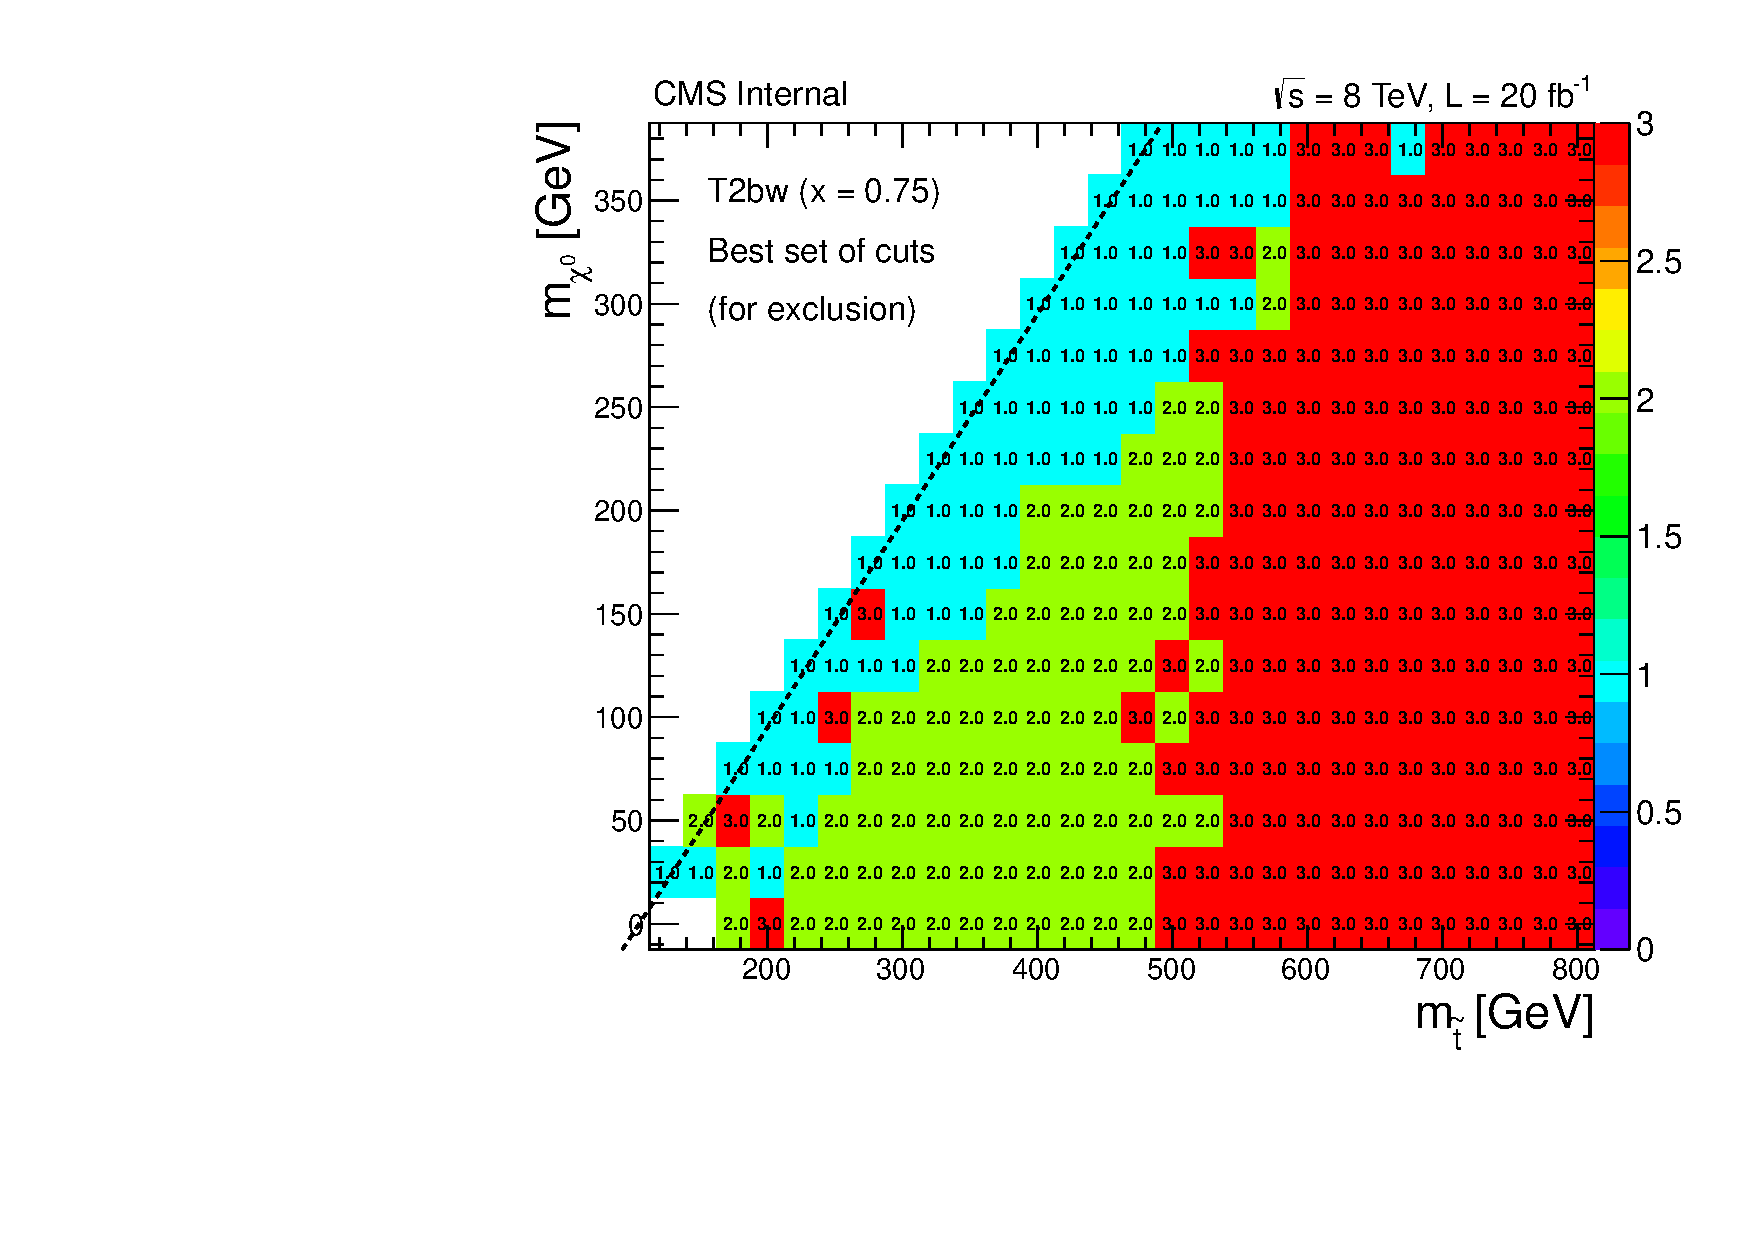
\includegraphics[width=0.36\textwidth]{cutAndCountPerformances/bestSet_T2bw075}
                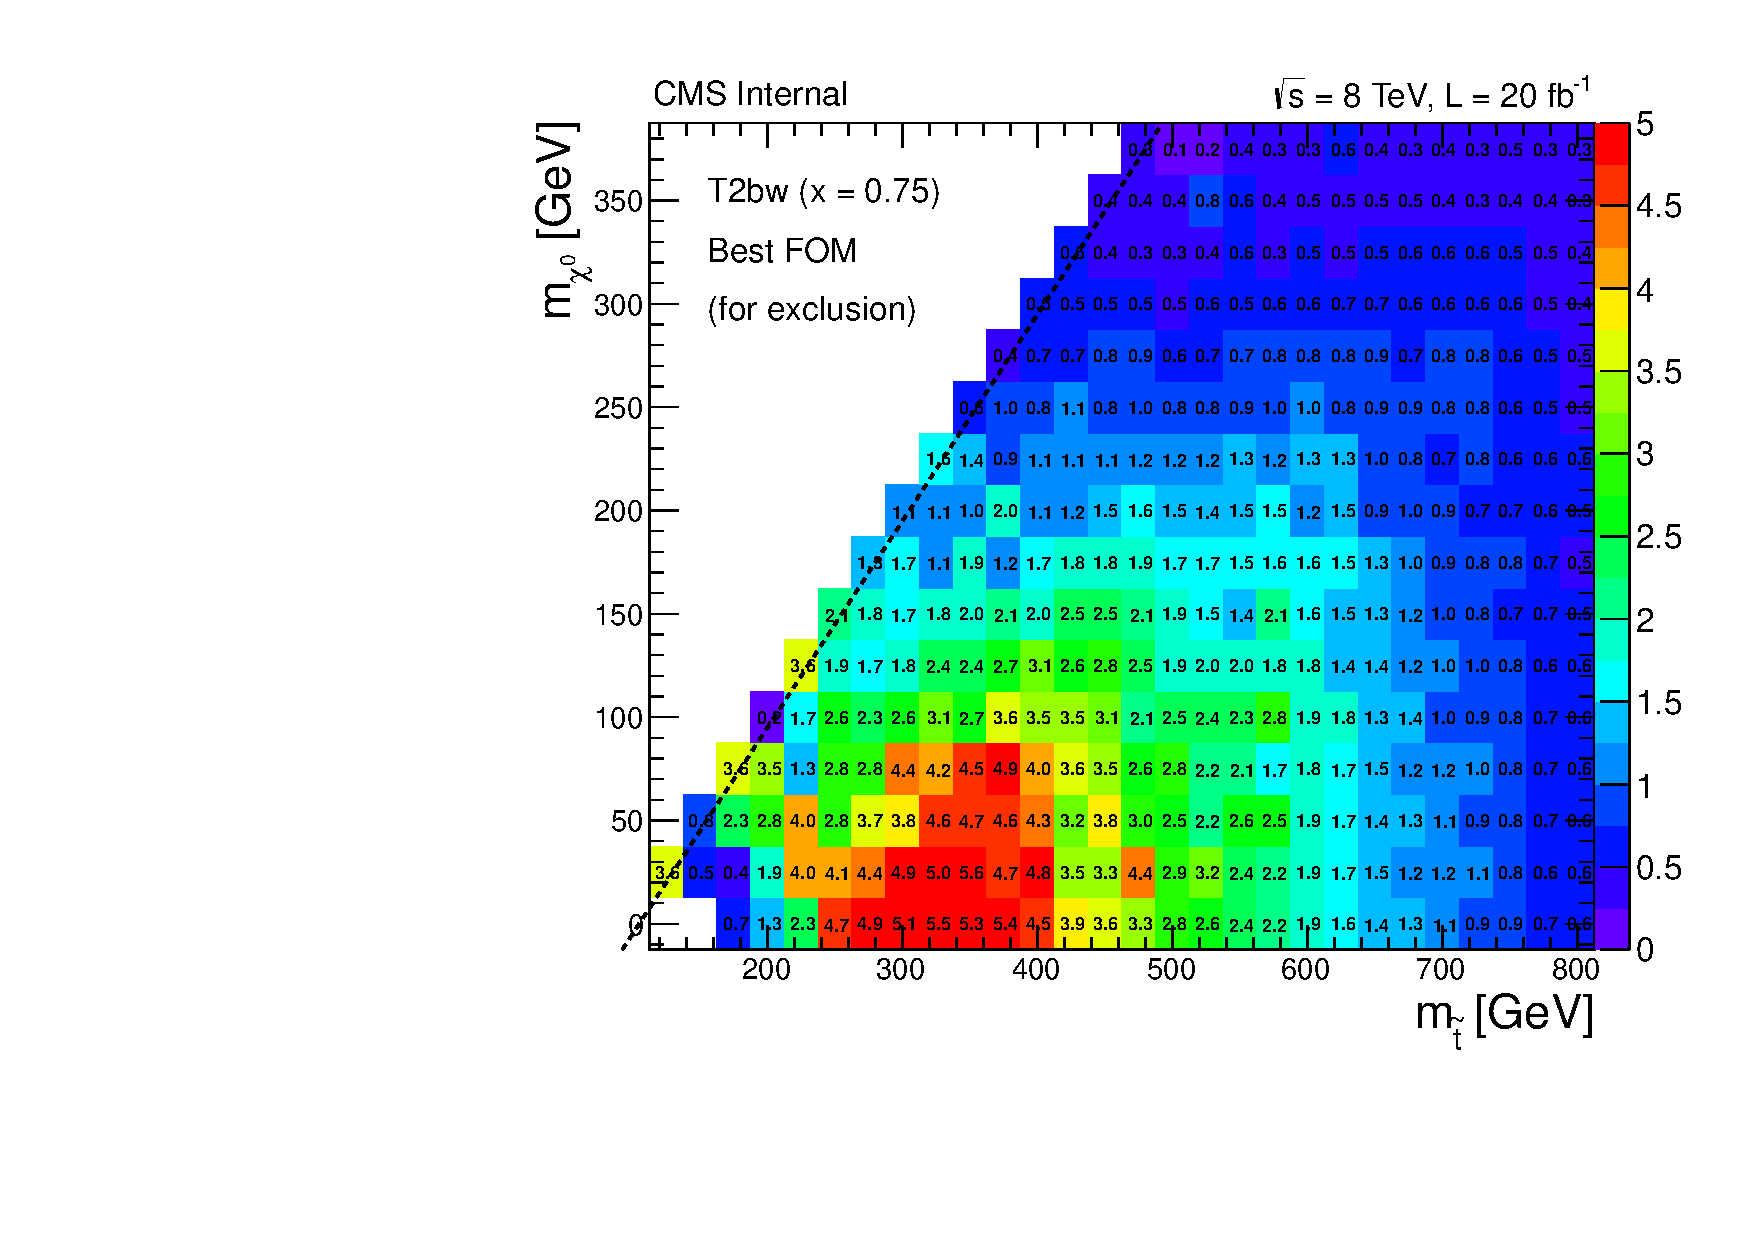
\includegraphics[width=0.36\textwidth]{cutAndCountPerformances/bestFOM_T2bw075}\\
                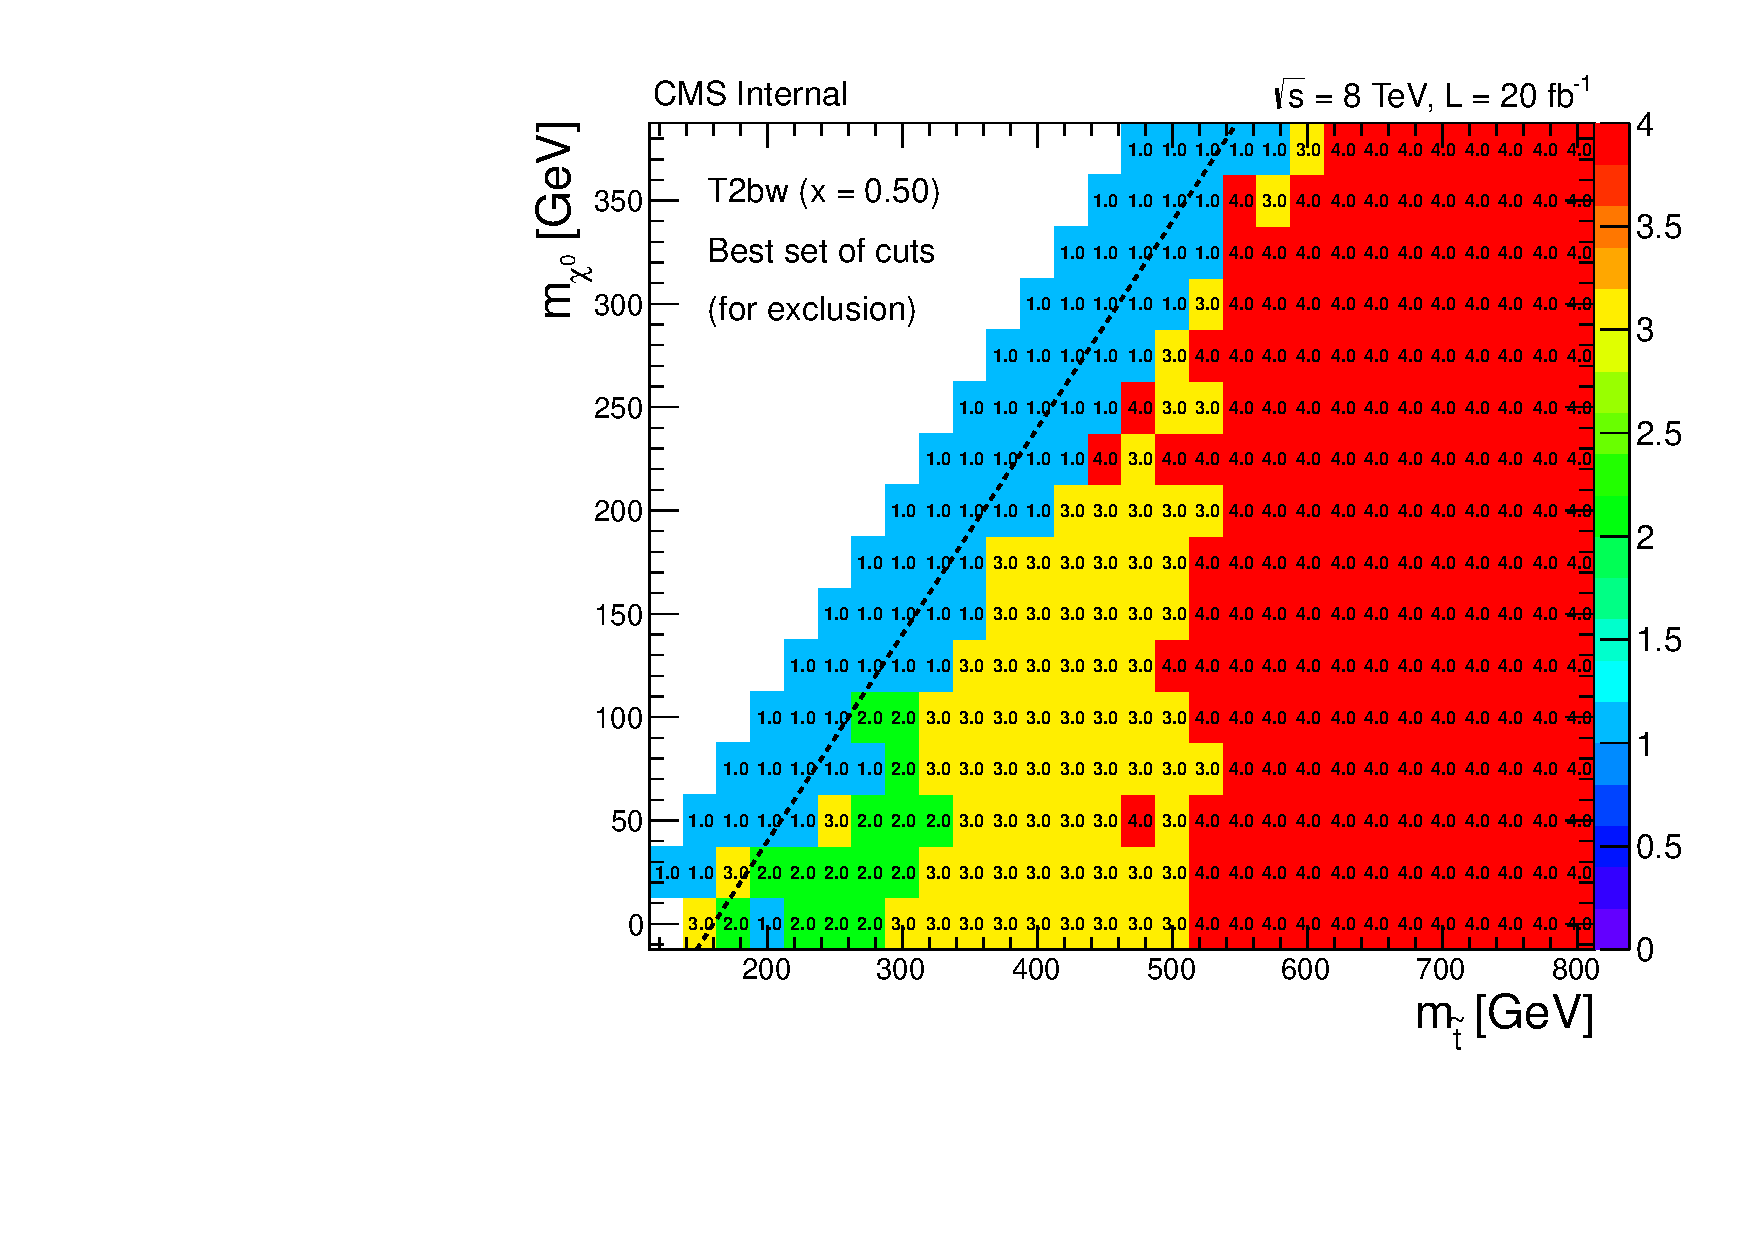
\includegraphics[width=0.36\textwidth]{cutAndCountPerformances/bestSet_T2bw050}
                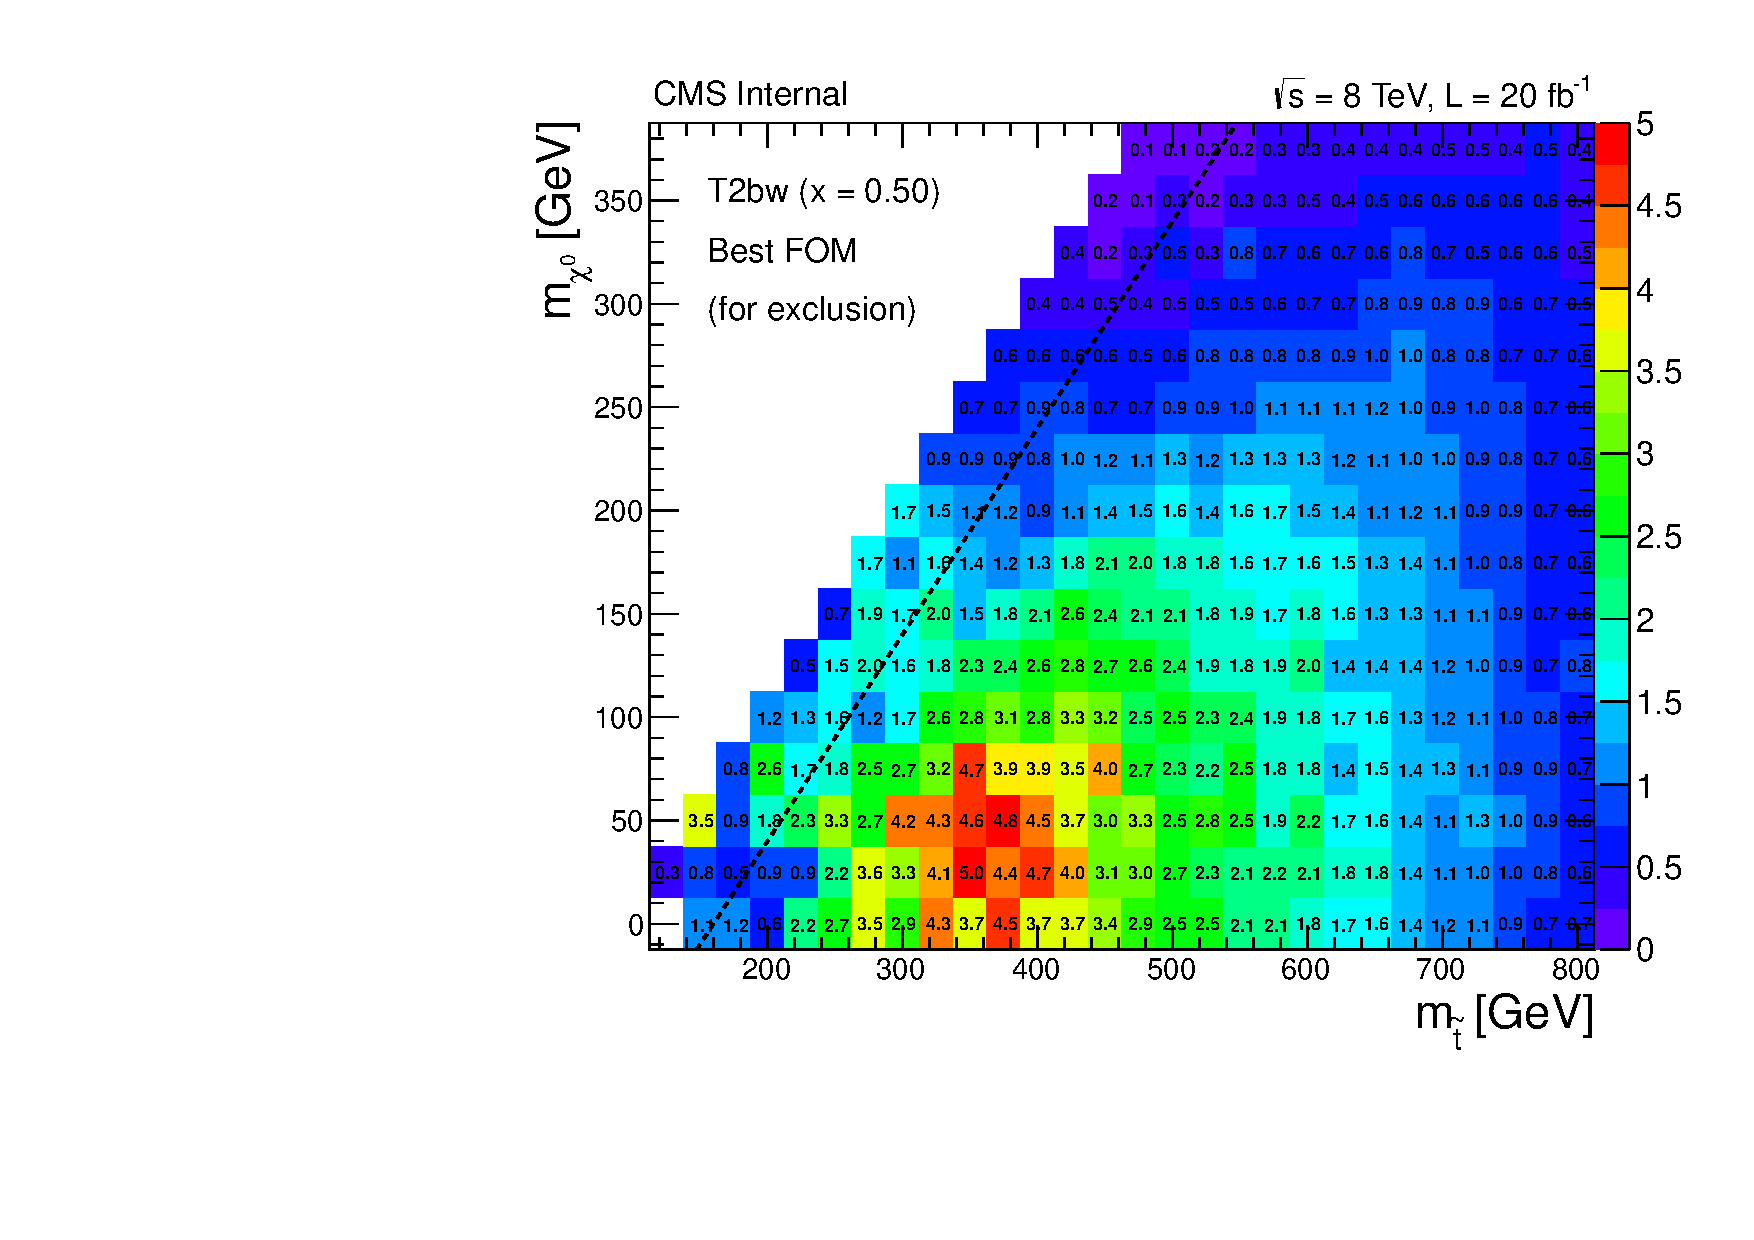
\includegraphics[width=0.36\textwidth]{cutAndCountPerformances/bestFOM_T2bw050}\\
                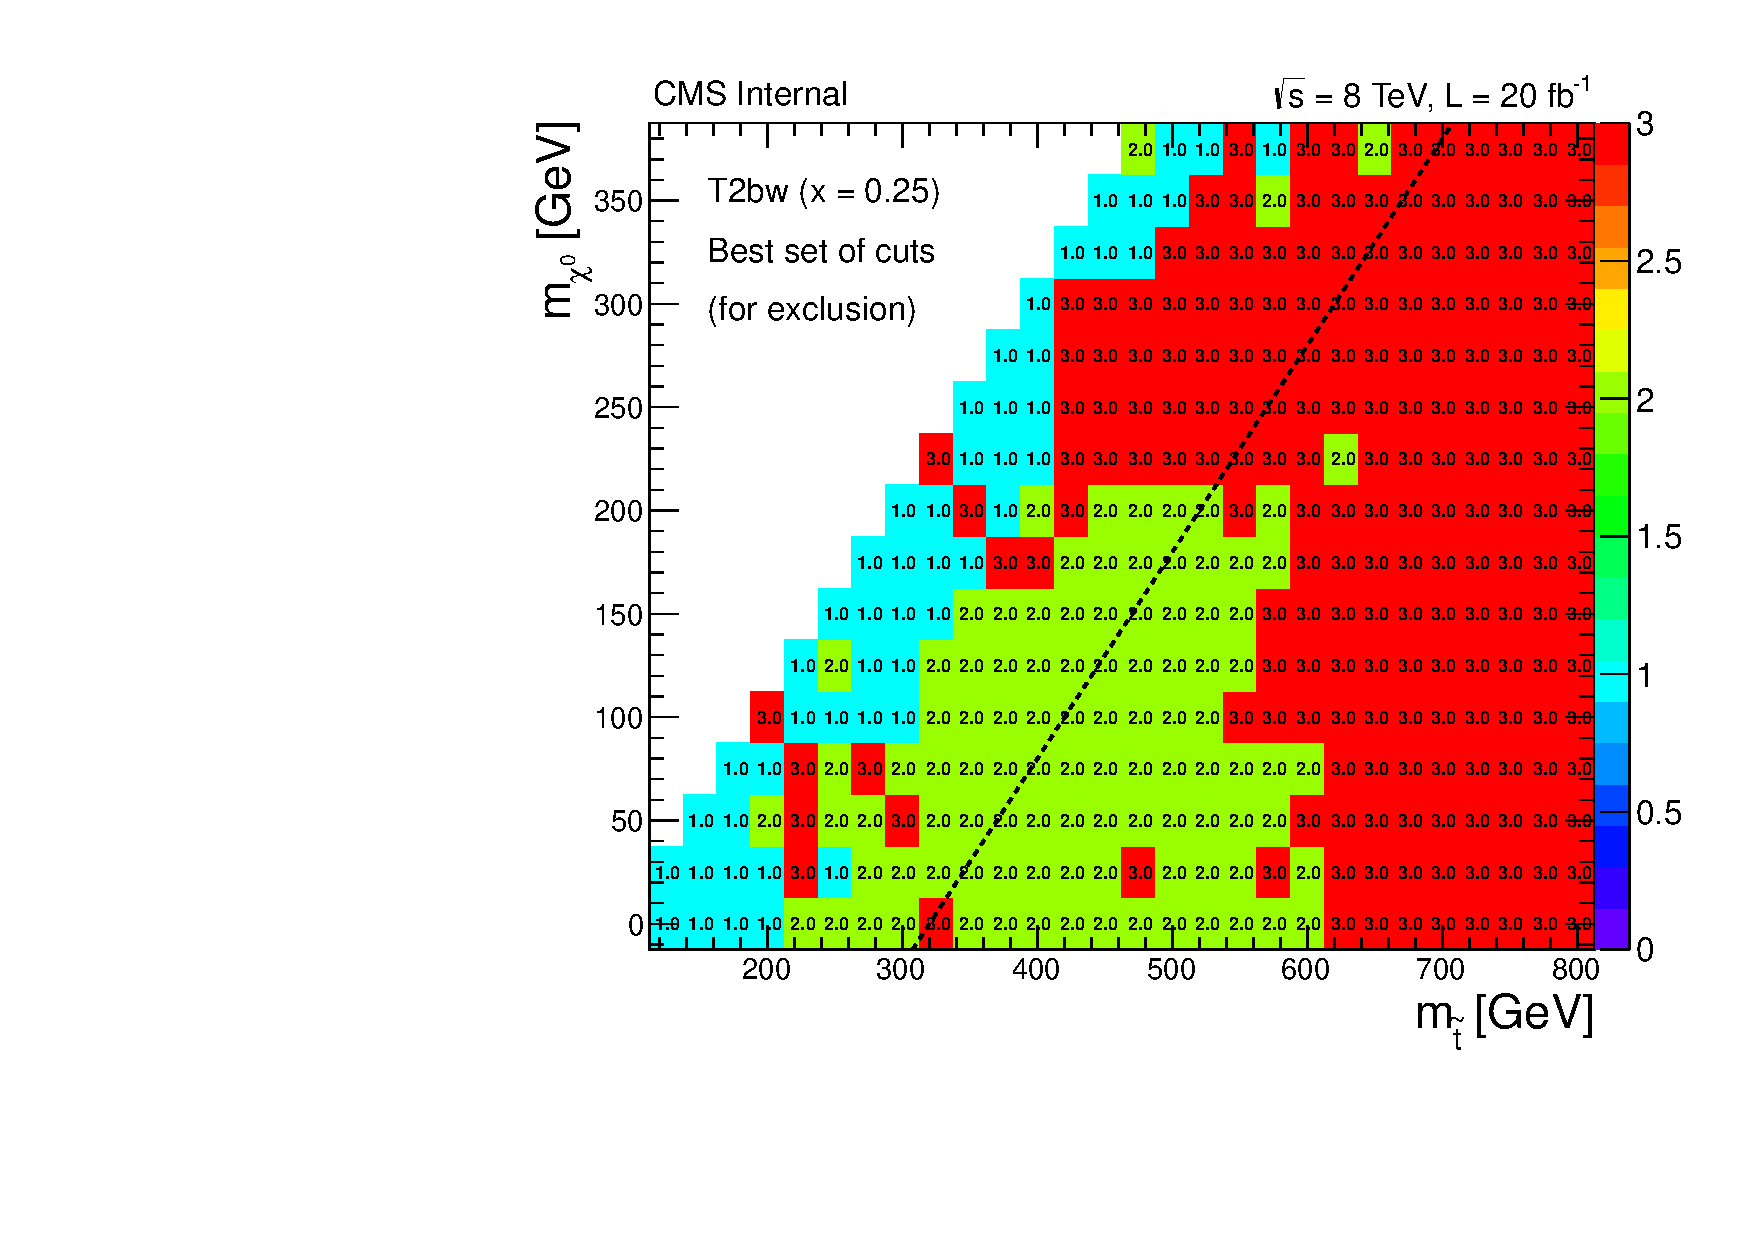
\includegraphics[width=0.36\textwidth]{cutAndCountPerformances/bestSet_T2bw025}
                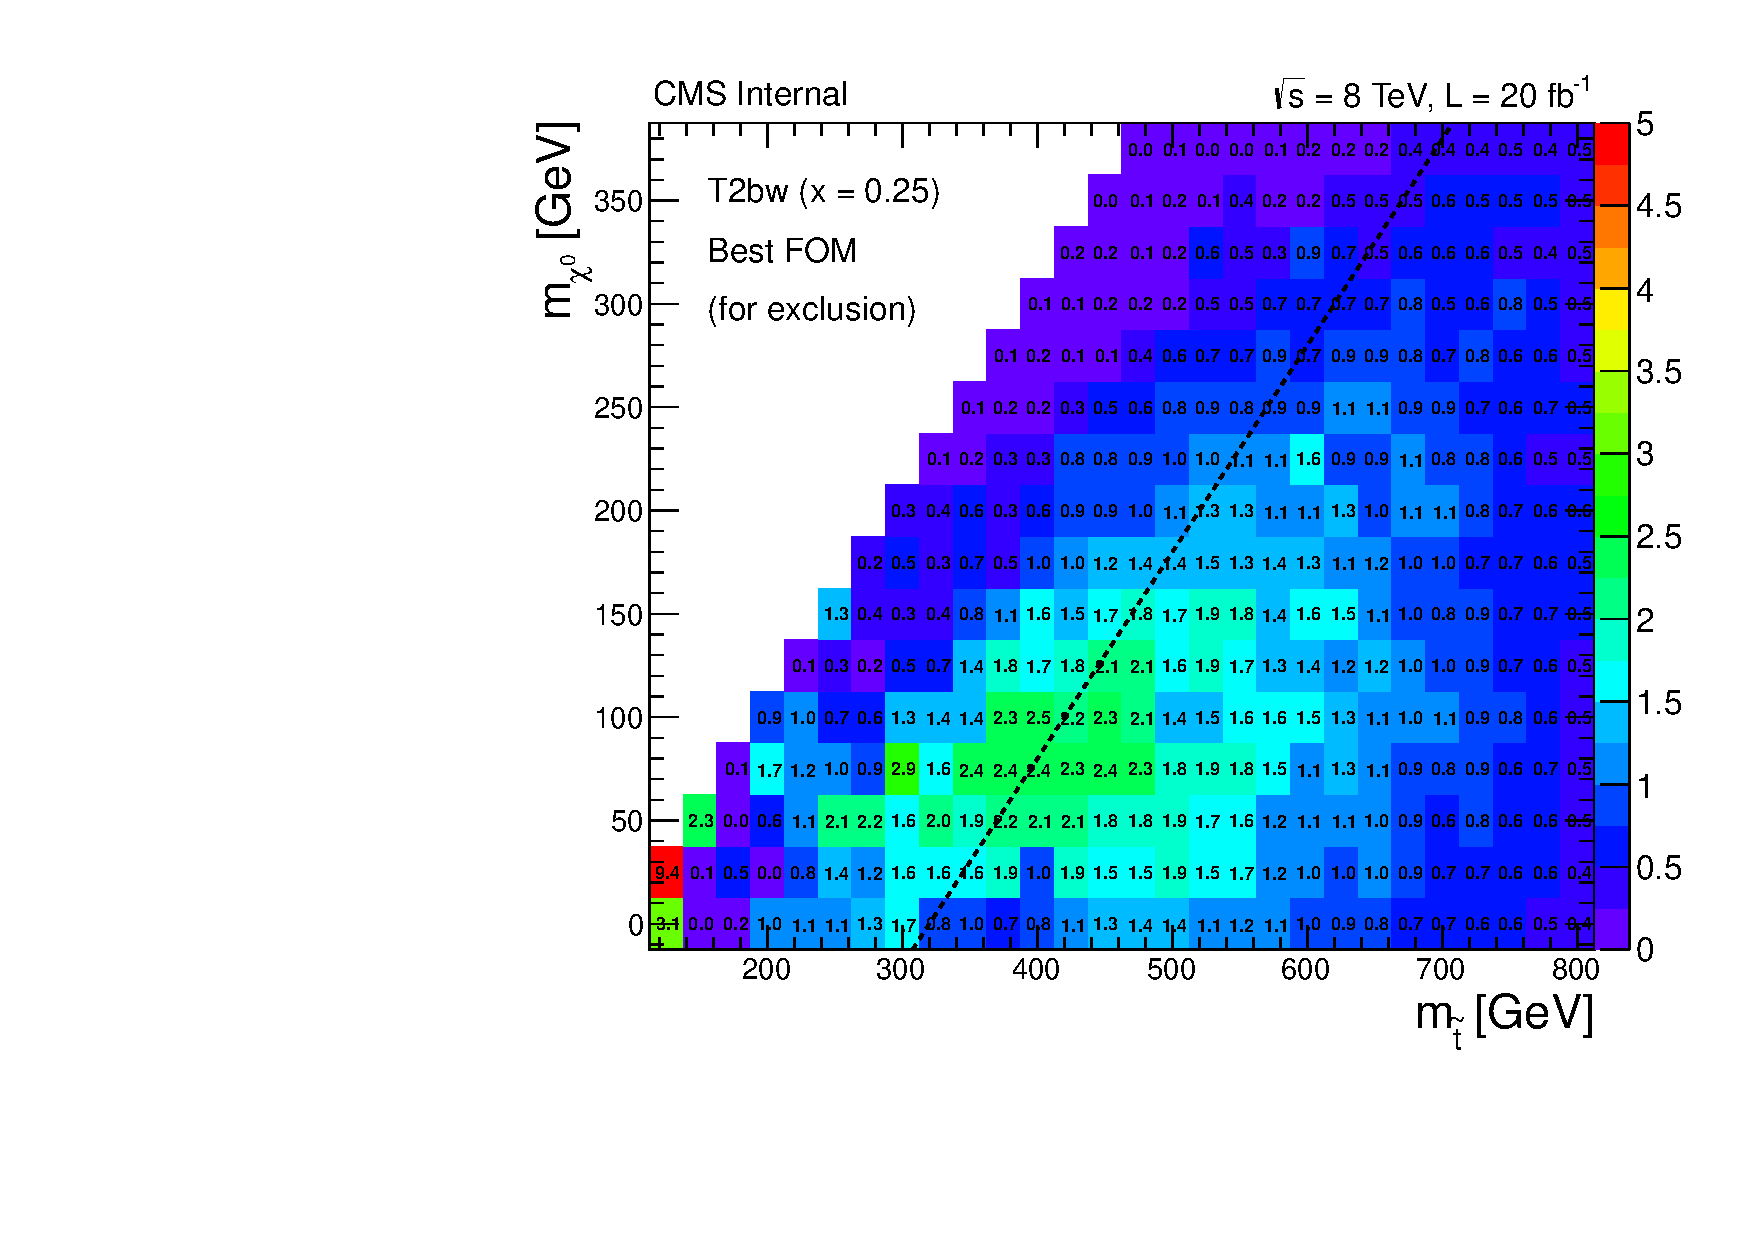
\includegraphics[width=0.36\textwidth]{cutAndCountPerformances/bestFOM_T2bw025}
                \caption{Best set of cuts (on the left) and performances in term of FoM$_\text{exclusion}$ (on the right) for the $\lstop \rightarrow t \lneutralino$ decay mode (first row) and $\lstop \rightarrow b \lchargino$ decay mode with x = 0.75 (second row), 0.50 (third row) and 0.25 (last row).}                                                     
                \label{fig:cutAndCountPerformances}
            \end{figure}

        \subsection{BDT-based signal regions}
        
            For the multivariate approach, several BDT are trained on slices of $\deltam$ in the $(\mass{\lstop},\mass{\lneutralino})$
            space against the $t\bar{t}$ background only. The choice of the variable is driven by an iterative method where variables 
            are added to BDT and kept if the performances are overall significantly improved across different slices of $\deltam$. The 
            performances of the BDTs are quantified by optimizing the cut on the BDT output with respect to a discovery-oriented 
            FoM, considering all the background and assuming a relative systematic uncertainty of 15\%.

            The set of variables used are presented on Table \ref{tab:BDTVariableUsage} as function of the decay mode. The definition
            of the training region in the $(\mass{\lstop},\mass{\lneutralino})$ is then being looked at, noticing that some of the
            $\deltam$ slices can be merged together as the performances of the training are similar, essentially because the kinematic
            is not strongly different when moving from one slice to the other. The optimization of the cut on the BDT output is then
            performed by iteratively looking at the excluded cross-section after the full procedure explained in the following sections.
            The cuts are tuned manually to optimize the sensitivity accordingly. Here, because of the cross-section regimes leading to 
            different amount of signal statistics, it is noticed that there is sometimes a significant gain in loosening or tightening
            the cut inside a same training region.

            The final definition of the training regions is presented on Figure \ref{fig:BDTTrainingRegions}. Each number represent a 
            different BDT training. The dashed lines represent the cases when one training region leads to several cut applied to define
            signal regions.

            \begin{table}[h!]
                \begin{center}
                    \begin{tabular}{|c|cc|ccc|}
                        
                        \hline
                        Variable                            & T2tt      & T2tt      & T2bw      & T2bw      & T2bw      \\
                                                            & off-shell & on-shell  & $x=0.25$  & $x=0.50$  & $x=0.75$  \\
                        \hline
                        $MET$                               &     x     &     x     &     x     &     x     &     x     \\ 
                        $M_{T2}^W$                          &           &     x     &     x     &     x     &     x     \\
                        $M_{\ell b}$                        &     x     &           &     x     &     x     &     x     \\
                        $M_{3 b}$                           &           &           &     x     &     x     &     x     \\
                        $\pT(\text{lead. } \ell)$           &     x     &     x     &     x     &     x     &     x     \\   
                        $\pT(\text{lead. } b)$              &     x     &           &     x     &     x     &           \\
                        $\pT(\text{lead. jet})$             &           &     x     &           &           &     x     \\
                        $H_{T}$                             &           &           &           &           &     x     \\
                        $H_{T}^\text{ratio}$                &     x     &     x     &           &           &           \\   
                        hadronic top $\chi^2$               &           &     x     &           &           &           \\
                        $\Delta\phi(j_{1,2},\vec{MET})$     &     x     &     x     &     x     &     x     &     x     \\
                        $\Delta R( \ell, \text{lead. } b)$  &           &     x     &           &     x     &           \\
                        $N_\text{jets}$                     &     x     &     x     &     x     &     x     &     x     \\
                        \hline
                    \end{tabular}
                    \caption{Use of the variables in the training of the BDT as function of the decay mode}
                    \label{tab:BDTVariableUsage}
                \end{center}
            \end{table}

            \insertFourFigures{BDTTrainingRegions}
                              {BDT/training_T2tt}
                              {BDT/training_T2bw075}
                              {BDT/training_T2bw050}
                              {BDT/training_T2bw025}
                              {0.49}
                              {Slicing of the $(\mass{\lstop},\mass{\lneutralino})$ space to define the training region of the BDTs. Some training regions are subdivised into subregions where different cuts are applied on the BDT output in order to adapt the sensitivity to the local cross-section.}

    \section{Background estimation \label{sec:analysis_backgroundEstimation}}

        \subsection{Overview} 

        In this section, we focus on the estimation of the different background contributions. 
        Four kinds of control regions are defined by inverting some of the requirements of the
        preselection and signal regions, as illustrated on Figure \ref{fig:backgroundEstimationOverview}.
        Each of these aim to provide signal-free sectors in which to check how good is the modeling
        of the backgrounds by the Monte-Carlo and perform data-driven estimations.

            \insertFigure{backgroundEstimationOverview}{0.7}
                         {Overview of the control regions used in the background estimation method.}

        The $\MT$-peak control region is defined by looking at events satisfying $50 < \MT < 80 \GeV$
        instead of the signal region $\MT$ requirement. This control region is enriched in $\oneLeptonTop$
        and is used as a well-controled region in which to normalize the $\oneLeptonTop$, $\Wjets$ 
        and $\diLeptonTop$ as documented in \ref{sec:MTpeakNormalization}.
        
        The $0b\text{-tag}$ control region is defined by requiring no $b$-tagged jet in the event.
        This region is enriched in $\Wjets$ and $\oneLeptonTop$ and is used to control and correct 
        the tail of $\MT$ for these two components as described in \ref{sec:MTtailCorrection}.

        The $2\ell$ control region is defined by requiring exactly two selected leptons instead of
        one, and lowering the $MET$ cut to $50 \GeV$. Additionnally, to limit the contribution
        from Drell-Yan, we veto events where the invariant mass of the dilepton system, $\mass{\ell\ell}$,
        is such that $\left|\mass{\ell\ell} - m_{Z}\right| < 15 \GeV$. Finally, the $1\ell$+veto control 
        region is defined by requiring exactly one selected leptons and one lepton veto. This region 
        is intended to control the modeling of the second lepton veto. Both the $2\ell$ and $1\ell$+veto
        are being looked at on the whole $\MT$ range and are not used to derive scale factors but only 
        systematic uncertainties on the background as detailed in \ref{sec:background_systematics}.

        Table \ref{tab:cutflowControlRegions} shows a breakdown of the background contributions in the 
        different control regions at the preselection level.

        \begin{table}[h!]
        \begin{tabular}{|c|cccc|}
            \hline
                             & $\MT$-peak             & $0b$-tag               & lepton+veto            & 2 leptons             \\ 
            \hline
             $\oneLeptonTop$ & 18523.00 $\pm$ 55.67   &  1213.32 $\pm$ 14.32   &  7030.10 $\pm$ 34.21   &   41.48 $\pm$ 2.71    \\  
             $\diLeptonTop$  &   656.73 $\pm$ 10.57   &   382.12 $\pm$ 8.05    &  7066.67 $\pm$ 34.44   & 9211.93 $\pm$ 39.65   \\
             $\Wjets$        &  1470.22 $\pm$ 24.62   &  2669.16 $\pm$ 33.54   &   331.25 $\pm$ 11.42   &    2.06 $\pm$ 0.93    \\ 
             rare            &  1209.69 $\pm$ 23.47   &   198.33 $\pm$ 7.45    &  1093.59 $\pm$ 20.25   &  626.57 $\pm$ 15.61   \\
            \hline
             total SM        & 21859.63 $\pm$ 66.09   &  4462.92 $\pm$ 38.09   & 15521.61 $\pm$ 53.82   & 9882.05 $\pm$ 42.70   \\ 
            \hline
        \end{tabular}
            \caption{Breakdown of the yield of the different background categories and for the four control regions.}
            \label{tab:cutflowControlRegions}
        \end{table}

        \subsection{Background normalization in $\MT$-peak \label{sec:MTpeakNormalization}}

            The $\MT$-peak control region, defined as $50 < \MT < 80 \GeV$ is the first step of the
            background estimation method. It is used to normalize the $\oneLeptonTop$, $\Wjets$ and
            $\diLeptonTop$ components while the rare component is taken directly from Monte-Carlo.
            This normalization is done for each signal region individually, effectively allowing to
            absorb disagreements caused by cuts on not-so-well modeled variables and uncertainty on the
            je energy scale, the trigger efficiency, lepton identification efficiency and luminosity.

            The normalization is done in two steps : first, a scale factor $\SFpre$ is
            computed before the application of the second lepton veto, substracting the rare component :

            \begin{equation}
                \SFpre \definedAs \left( \frac{N(\text{data}) - N(\text{rare})}{N(\oneLeptonTop) + N(\Wjets) + N(\diLeptonTop)} \right)
                \label{eq:SFpreDefinition}
            \end{equation}

            $\SFpre$ is used to normalize only the $\diLeptonTop$ component. Another scale factor, $\SFpost$ is used after application of the second lepton veto, substracting the rare and the corrected $\diLeptonTop$ component :

            \begin{equation}
                \SFpost \definedAs \left( \frac{N(\text{data}) - N(\text{rare}) - \SFpre \times N(\diLeptonTop)}{N(\oneLeptonTop) + N(\Wjets)} \right)
                \label{eq:SFpostDefinition}
            \end{equation}

            At preselection level, $\SFpre$ and $\SFpost$ are equal to $(1.06 \pm 0.01)$ and $(1.05 \pm 0.01)$ respectively.

        \subsection{$\MT$-tail correction in the $0b$-tag region \label{sec:MTtailCorrection}}

        The $0b$-tag control region allows to control the tail of $\MT$ of the $\Wjets$ and $\oneLeptonTop$ components. Before looking at the tail, however, we start by normalizing the background in the $\MT$ peak of this control region, in a similar fashion as what is done in \ref{sec:MTpeakNormalization}. This is done by introducing $\SFnobtag$, used to normalize the $\Wjets$ and $\oneLeptonTop$ contributions :

        \begin{equation}
            \SFnobtag \definedAs \left( \frac{N(\text{data}) - N(\text{rare}) - N(\diLeptonTop)}{N(\oneLeptonTop) + N(\Wjets)} \right)
            \label{eq:SF0btagDefinition}
        \end{equation}

        At preselection level, $\SFnobtag$ is found to be $(0.99 \pm 0.01)$. After normalization to the peak, a clear disagreement in the tail of $\MT$ is observed for $\MT > 100 \GeV$ between the data and Monte-Carlo, as shown on \ref{fig:templateFit/MT_notCorrected}. This is an important point of the analysis as it means that the Monte-Carlo needs to be corrected to have a reliable prediction of the $\oneLeptonTop$ and $\Wjets$ in the $\MT$ tail. So far, the understanding of this disagreement comes from two source : first, the off-shell contributions of $\Wjets$ is underestimated by the simulation, and second, detector effects leads to a larger tail for the $\oneLeptonTop$ events.

        \insertFigure{templateFit/MT_notCorrected}{0.7}
                     {Data/MC comparison on the full $M_T$ distribution in the $0b$-tag control region at preselection level, after propagation of $\SFnobtag$. A clear discrepancy is visible for $\MT > 100 \GeV$.}

        A method is put in place to correct the discrepancy using a template fit to estimate separately the contribution of $\oneLeptonTop$ and $\Wjets$ from the data. To do this, we use $\MlbPrime$ which was found to have a good discriminating power between the two process categories and being well discribed in the peak of $\MT$, as shown on \ref{fig:MlbPrimeForTemplateFit}.

        \insertFourFigures{MlbPrimeForTemplateFit}
                          {templateFit/Mlb_0b_peak}
                          {templateFit/Mlb_0b_tail}
                          {templateFit/preselection_Mlb_noFit}
                          {templateFit/preselection_Mlb_withFit}
                          {0.45}
                          {Distribution of $\MlbPrime$ in the $0b$-tag control region, data/MC comparison in the $M_T$ peak (top left), superimposed and normalized $\oneLeptonTop$ and $\Wjets$ components in the $M_T$ tail (top right), data/MC comparison in the $M_T$ tail before correction of the Monte-Carlo (bottom left) and after correction (bottom right). On the bottom right, the uncertainty of the scale factors are propagated in the ratio.}

        The method is implemented using the \textsc{RooFit} toolbox with the Minuit2 implementation of the \textsc{Migrad} minimizer algorithm. The normalization of the $\oneLeptonTop$ and $\Wjets$ components are free parameters translated in term of scale factors, $SF_{\oneLeptonTop}$ and $SF_{\Wjets}$, while the normalization of the $\diLeptonTop$ and rare components are taken from the Monte-Carlo and constrained with a 20\% uncertainty during the fit process. To validate the method, a closure test is performed by generating toy data from the Monte-Carlo where arbitrary scale factors where injected. The estimated scale factors are then compared to the input scale factors. A very good linearity is found for scale factors varying from 0.10 to 3. The fit is performed both in the $\MT$ peak and tail regions and we extract $SFR = SF^{\text{tail}} / SF^{\text{peak}}$ for both processes, representing the discrepancy in the tail independently from the peak normalization. Different sources of systematic uncertainty are considered : the jet energy scale, the normalization of the rare background, the Monte-Carlo statistics, the choice of the minimizer algorithm, the choice of the initial fit conditions, the generator setup (scale, matching, top pass, \textsc{Powheg} or \textsc{MadGraph}, top $\pT$ reweighting). The most important sources are the Monte-Carlo statistics (leading to 11\% of relative uncertainty on SFR), the generator scale (9\%) and the jet energy scale. A conservative 20\% is used as relative systematic uncertainty.

        At preselection level, $\SFRoneLeptonTop$ and $\SFRWjets$ are found to be $(1.04 \pm 0.16 (\text{stat.}) \pm 0.21 (\text{syst.}))$ and $(1.33 \pm 0.10 (\text{stat.}) \pm 0.27 (\text{syst.}) )$ respectively. The plot on Figure \ref{fig:MlbPrimeForTemplateFit} illustrate the impact on the $\MlbPrime$ data/MC comparison after propagating the scale factors.

        To be as close as possible to the kinematic of the signal region, one would like to perform the template fit method directly in the signal region. It is however not possible as the statistics is too low. To work around this problem, relaxed BDT signal regions are built by loosening the cut on the BDT output such as at least 25\% of the background is still selected. The template fit method is performed in these relaxed BDT signal region. The resulting $\SFRoneLeptonTop$ and $\SFRWjets$ are represented on Figure \ref{fig:templateFitBDTResults}. The value actually used is an average across all the BDT training as represented by the red line and corresponds to $\SFRoneLeptonTop = (1.38 \pm 0.61)$ and $\SFRWjets = (1.21 \pm 0.36)$.

        For the cut-based signal regions, we use the scale factors derived from a single $M_T$ cut associated to the signal region as shown on Figure \ref{fig:templateFitCnCResults} on the left. To cover possible correlation between the $SFR$ and $MET$, the uncertainty from the single $MET$ or $MET/\sqrt{H_T}$ associated to the signal region is also quadratically added to the scale factor.

        \insertTwoFigures{templateFitBDTResults}
                          {templateFit/BDT_1ltop}
                          {templateFit/BDT_Wjets}
                          {0.7}
                          {Template fit results for $\oneLeptonTop$ (top) and $\Wjets$ (bottom) for the different BDT discriminators, keeping 25\% of the statistics after the cut. The uncertainty is only statistical. The red line represents the mean value for the $SFR$ and the blue dotted lines account for the uncertainty on the $SFR$.}

        \insertThreeFigures{templateFitCnCResults}
                           {templateFit/CnC_MTcuts}
                           {templateFit/CnC_METcuts}
                           {templateFit/CnC_METoverSqrtHTcuts}
                           {0.325}
                           {Template fit results for individual cuts on $\MT$ (left), $MET$ (middle) and $MET/\sqrt{H_T}$ (right) after preselection. The uncertainties shown are statistical only.}
        
        \subsection{Control of the second lepton veto and $\diLeptonTop$ component}

        The 2 lepton and lepton+veto control regions allow to check for the good modeling of the $\diLeptonTop$ background and the second lepton veto definition. The $\MT$-peak of the lepton+veto control region is dominated by $\oneLeptonTop$ where a fake second lepton was reconstructed while the $\MT$-tail is dominated by $\diLeptonTop$ with a true second lepton. As for the $\MT$-peak normalization, we introduce scale factors to normalize the backgrounds in the peak of $\MT$ and quantify the agreement in the tail. 

        In the lepton+veto region, we define $\SFveto$ in a similar fashion as $\SFpost$ :

        \begin{equation}
            \SFveto \definedAs \left( \frac{N(\text{data}) - N(\text{rare}) - \SFpre \times N(\diLeptonTop)}{N(\oneLeptonTop) + N(\Wjets)} \right)
        \end{equation}

        $\SFveto$ is used to normalize the $\oneLeptonTop$ and $\Wjets$ components to the peak. From that, we define $\SFvetoTail$ by propagating $\SFpre$ and $\SFpost$ but also $\SFRoneLeptonTop$ and $\SFRWjets$ in the tail :

        \begin{equation}
            \hspace*{-1.5cm}
            \SFvetoTail \definedAs \left( \frac{N(\text{data}) - N(\text{rare}) - \SFveto \times \SFRoneLeptonTop \times N(\oneLeptonTop) - \SFveto \times \SFRWjets \times N(\Wjets)}{ \SFpre \times  N(\diLeptonTop)} \right)
        \end{equation}

        At preselection level, we find $\SFveto = (1.18 \pm 0.03)$ and $\SFvetoTail = (1.07 \pm 0.02)$.

        In the 2 leptons control region, we define

        \begin{equation}
            \SFtwoLep \definedAs \left( \frac{N(\text{data}) - N(\text{rare})}{N(\diLeptonTop) + N(\oneLeptonTop) + N(\Wjets)} \right)
        \end{equation}

        and 

        \begin{equation}
            \SFtwoLepTail \definedAs \left( \frac{N(\text{data}) - N(\text{rare}) - \SFtwoLep \times (N(\oneLeptonTop) + N(\Wjets))}{\SFtwoLep \times N(\diLeptonTop)} \right)
        \end{equation}

        At preselection level, we find $\SFtwoLep = (0.96 \pm 0.01)$ and $\SFtwoLepTail = (1.01 \pm 0.02)$.

        Figure \ref{fig:preselMT2leptonAndLepPlusVeto} presents the full $\MT$ distributions for the lepton+veto and two leptons control region.

        \begin{figure}[h!]
            \centering
            \includegraphics[width=0.45\textwidth]{controlPlots/reversedVeto_noMTCut/MT}
            \includegraphics[width=0.45\textwidth]{controlPlots/2leptons_noMTCut/MT}
            \caption{Full $\MT$ distributions for the lepton+veto control region (on the left) and two leptons control region (on the right). On the left, $\SFpre$, $\SFveto$, $\SFRoneLeptonTop$ and $\SFRWjets$ are propagated. On the right, no scale factors is applied.}
                    \label{fig:preselMT2leptonAndLepPlusVeto}
        \end{figure}

        \subsection{Control plots at preselection level}

        Figure \ref{fig:preselControlPlots} shows control plots for $\MT$, $MET$ and $M_{T2}^W$ in the different control regions at the preselection level.

            \begin{figure}[h!]
                \centering
                \includegraphics[width=0.325\textwidth]{controlPlots/MTpeak/MT}
                \includegraphics[width=0.325\textwidth]{controlPlots/MTpeak/MET}
                \includegraphics[width=0.325\textwidth]{controlPlots/MTpeak/MT2W}\\
                \includegraphics[width=0.325\textwidth]{controlPlots/0btag/MT}
                \includegraphics[width=0.325\textwidth]{controlPlots/0btag/MET}
                \includegraphics[width=0.325\textwidth]{controlPlots/0btag/MT2W}\\
                \includegraphics[width=0.325\textwidth]{controlPlots/reversedVeto/MT}
                \includegraphics[width=0.325\textwidth]{controlPlots/reversedVeto/MET}
                \includegraphics[width=0.325\textwidth]{controlPlots/reversedVeto/MT2W}\\
                \includegraphics[width=0.325\textwidth]{controlPlots/2leptons/MT}
                \includegraphics[width=0.325\textwidth]{controlPlots/2leptons/MET}
                \includegraphics[width=0.325\textwidth]{controlPlots/2leptons/MT2W}\\
                \caption{A few control plots, showing the data/MC comparison for $\MT$ (left column), 
                        $MET$ (middle column) and $M_{T2}^W$ (right column) in the different control
                        regions : $\MT$-peak (first row), $0b$-tag (second row), 1 lepton+veto (third
                        row) and 2 leptons (fourth row). The $\MT$-peak normalization and $\MT$-tail
                        correction scale factors are propagated where relevant.}
                        \label{fig:preselControlPlots}
            \end{figure}

        \subsection{Background prediction}

        The background prediction is obtained by taking the Monte-Carlo yield in the $\MT$-tail and propagating $\SFpre$ to the $\diLeptonTop$ component and $\SFpost$ to the $\oneLeptonTop$ and $\Wjets$ component. The $\oneLeptonTop$ and $\Wjets$ are also corrected with $\SFRoneLeptonTop$ and $\SFRWjets$ respectively. The prediction for the rare component is directly the Monte-Carlo yield in $\MT$-tail. The formula \ref{eq:prediction1ltop} to \ref{eq:predictionrare} below summarize the computation of the prediction. The procedure is repeated for each signal region. As an illustration, Table \ref{tab:predictionPreselection} shows the comparison between the raw Monte-Carlo and the prediction obtained at preselection level.

        \begin{eqnarray}
            N^\text{pred}_\text{tail}(\oneLeptonTop) & = & N^\text{MC}_\text{tail}(\oneLeptonTop)  \times \SFpost \times \SFRoneLeptonTop \label{eq:prediction1ltop}  \\
            N^\text{pred}_\text{tail}(\Wjets)        & = & N^\text{MC}_\text{tail}(\Wjets)         \times \SFpost  \times \SFRWjets                             \\
            N^\text{pred}_\text{tail}(\diLeptonTop)  & = & N^\text{MC}_\text{tail}(\diLeptonTop)   \times \SFpre                                                \\
            N^\text{pred}_\text{tail}(\text{rare})   & = & N^\text{MC}_\text{tail}(\text{rare})                                           \label{eq:predictionrare} 
        \end{eqnarray}

        \begin{table}[!h]
            \begin{center}
                \begin{tabular}{|l|c|c|}
                    \hline
                                             &  \textbf{Raw MC}          & \textbf{Prediction}       \\
                    \hline
                    \textbf{$\oneLeptonTop$} &  5970.82 $\pm$ 31.72      & 6526.91 $\pm$ 1632.45     \\
                    \textbf{$\diLeptonTop$}  &  2117.45 $\pm$ 18.93      & 2253.37 $\pm$ 229.91      \\
                    \textbf{$\Wjets$}        &  477.25  $\pm$ 13.95       & 669.72 $\pm$ 364.59       \\
                    \textbf{rare}            &  490.23  $\pm$ 13.99       & 490.23 $\pm$ 245.51       \\
                    \hline
                    \textbf{Total SM}        &  9055.74 $\pm$ 41.89      & 9940.22 $\pm$ 1666.39     \\
                    \hline
                \end{tabular}
                \caption{ Background prediction at the preselection level.}
                \label{tab:predictionPreselection}
            \end{center}
        \end{table}

    \section{Systematic uncertainties \label{sec:analysis_systematics}}
        
        This section describes the sources of systematics uncertainties that are considered for the background and the signal.

        \subsection{Systematic uncertainties on the background \label{sec:background_systematics}}

            \subsubsection{Second lepton veto efficiency}

            The uncertainty on the efficiency of the second lepton veto is propagated to the
            fraction of $\diLeptonTop$ events that have a second lepton in the acceptance. For
            the isolated track veto lepton, this is defined as having a second generated 
            $e/\mu$ or a one prong $\tau \rightarrow h$ with $\pT > 5 \text{ or } 10 \GeV$, 
            respectively, with $\abseta < 2.4$. This fraction is about 70\%. The uncertainty 
            for these events is 6\% and is obtained from tag-and-probe studies \refNeeded.
            Regarding the $\tau$ veto lepton, the events considered are those 
            with a hadronic $\tau$ in the acceptance, with true visible transverse energy $> 20 
            \GeV$ in $\abseta < 2.4$. This fraction is about $10 \sim 15 \%$ of the total. The 
            uncertainty on the efficiency of the $\tau$-ID algorithm is 7\%, taken from $\tau$ 
            group studies \refNeeded.

            \subsubsection{Modeling of $\diLeptonTop$}

            The goodness of the modeling of the $\diLeptonTop$ background is checked in the 2
            leptons and 1 lepton + veto control regions via the scale factors $\SFtwoLepTail$
            and $\SFvetoTail$. As the agreement has been checked to be overall good, no correction
            for the modeling of the tail is applied to $\diLeptonTop$ to compute the prediction
            from the Monte-Carlo. However, an uncertainty is propagated to the $\diLeptonTop$ yield 
            as a way to quantify the trust in the Monte-Carlo.

            Because the cuts defining the signal regions are sometimes very tight, they lead to
            small number of events in the corresponding control region. This has for consequence that
            $\SFtwoLepTail$ and $\SFvetoTail$ have very large uncertainties and conclusions are
            difficult to draw.

            To work around this problem while still probing the tail of $\MT$ near the signal
            region, we define loosened cuts to check these scale factors with more statistics.
            These cuts are designed by requiring to have at least 30 events remaining in the tail of
            $\MT$ for the 2 lepton control region, to keep the uncertainty in the range of 20$\sim$30\%.
            
            For the BDT signal regions, it is done by loosening the cuts on the BDT outputs with
            three different cuts on $N_\text{jets}$ : $\geq 2$, $\geq 3$ and $\geq 4$. This mean
            that we consider three kinds of loosened BDT cuts. Doing so allows to probe further the
            description of the tail of the BDT output via $N_\text{jets} \geq 2$ because the looser
            $N_\text{jets}$ requirement allows a tighter cut, while $N_\text{jets} \geq 4$ is closer
            to the actual preselection but with a looser cut on the BDT output. 

            For the cut-based approach, it is done by removing the conditions on $\Delta \phi( j_{1,2},
            \vec{MET} )$ and, hadronic top $\chi^2$ and the condition on $N_\text{jets}$ in the definition
            of the ISR-jet selection. For some of the signal regions, it is needed to go further by 
            relaxing the $MET$, $M_{T2}^W$ and $\pT(\text{lead.} b)$ cuts. 

            For each of the relaxed control region, we compute the value of $\SFtwoLepTail$ and
            $\SFvetoTail$ to quantify the agreement between data and the simulation in the tail of $\MT$.
            The scale factors are found to be compatible with one and and enveloppe is computed for
            each signal region to account for the spread of the scale factors for each of the
            associated control regions. The results are presented on \ref{fig:systematics/BDT_enveloppe} for
            the BDT signal regions.

            \insertFigure{systematics/BDT_enveloppe}{0.8}
                         {Illustration of the scale factors computed in the relaxed two leptons and lepton+veto control regions of each BDT signal region, as well as the enveloppe (in solid black) used to quantify the confidence in the good modeling of the $\diLeptonTop$ background.}

            \subsubsection{Modeling of $N_\text{jets}$ for $t\bar{t}$}

            As the $N_\text{jets}$ variable is used in the BDT signal region, one wants to test the
            capacity of the simulation to model this variable correctly. This can be done by
            studying the $t\bar{t}$ background in a two lepton control region. The different
            $N_\text{jets}$ bins allow to probe the production of ISR and FSR jets. In particular,
            the bins 2, 3 and $\geq$4 probe the production of 0, 1 and 2 additional jets and
            can be use to extract a scale factor to be applied on the $\oneLeptonTop$ components
            for the bin 4, 5 and $\geq$6. In the same way, the bins 4, 5 and 6 allow to derive
            a scale factor for the $\diLeptonTop$ component. 
            
            Table \ref{tab:NjetsModeling} present the scale factors obtained. As they are compatible
            with one, no correction factor is added but an uncertainty of 2\% is propagated.

            \begin{table}
                \centering
                \begin{tabular}{|c|c|}
                    \hline
                   $N_\text{jets}$ & scale factor \\
                    \hline
                    2              & $0.99 \pm 0.01$ \\
                    3              & $1.00 \pm 0.02$ \\
                    $\geq$4        & $1.02 \pm 0.02$ \\
                    \hline          
                    4              & $1.06 \pm 0.05$ \\
                    5              & $0.97 \pm 0.09$ \\
                    $\geq$6        & $0.84 \pm 0.15$ \\
                    \hline
                \end{tabular}
                \caption{Scale factors related to the $N_\text{jets}$ modeling for $t\bar{t}$ events in a 2 lepton region at preselection level.}
                \label{tab:NjetsModeling}
            \end{table}

            \subsubsection{Cross section of $\oneLeptonTop$, $\Wjets$ and rare components}
        
            The $\oneLeptonTop$ component cross-section is varied by 10\% while the $W$+jets 
            and rare background cross-sections are varied by 50\%. The uncertainty on the rare 
            component cross-section is meant to conservatively cover the knowledge we have of 
            this background as it taken directly from the Monte-Carlo, while the $\oneLeptonTop$ and 
            $\Wjets$ cross-sections uncertainty are meant to cover variations in the relative 
            proportions of the backgrounds. These uncertainty impact the normalization of the 
            other backgrounds during the $\MT$-peak normalization through $\SFpre$ and $\SFpost$.

            \subsubsection{Statistic uncertainty in $\MT$ peak}
            
            The statistics being limited in the $\MT$-peak region, the computation of 
            $\SFpre$ and $\SFpost$ comes with an uncertainty dominated by the event counts 
            in the data. The uncertainty is propagated to the total background yield uncertainty.

            \subsubsection{Uncertainty on $\SFRoneLeptonTop$ and $\SFRWjets$}

            As described in section \label{sec:MTtailCorrection}, the $\MT$-tail correction
            scale factors for $\oneLeptonTop$ and $\Wjets$ are computed with an uncertainty
            coming from statistics in the $0b$-tag control region and systematic effects
            from the template fit method itself. This uncertainty is propagated to the total
            background yield uncertainty and is one of the major contribution for the signal
            region with a large remaining fraction of $\oneLeptonTop$.

            \subsubsection{Limited statistic of the Monte-Carlo in $\MT$ tail}
            
            As the Monte-Carlo statistics is limited in the $\MT$ tail, the associated uncertainty
            is propagated when computing equations \ref{eq:prediction1ltop} to \ref{eq:predictionrare}.

            \subsubsection{Summary of background uncertainties at preselection}
           
            Table \ref{tab:systematicsPreselection} shows a breakdown of the different systematics
            uncertainties that are considered, at preselection level. It should be noted that the
            relative importance of the individual systematics varies depending of the signal regions
            as the composition of the background varies a lot. At preselection level, the importance
            of the $\SFRoneLeptonTop$ uncertainty is high as the $\oneLeptonTop$ component is still large.
            However for some signal regions, the $\diLeptonTop$ is the dominant contributions and
            uncertainty from the $\MT$-tail modeling is the leading systematic source.

            \begin{table}[!ht]
                \begin{center}
                    \begin{tabular}{|l|c|c|}
                        \hline
                        & \textbf{absolute} & \textbf{relative (\%)}   \\
                        \hline
                        \textbf{$\diLeptonTop$ ($\MT$-tail modeling)}       & 155.5    & 1.6  \\
                        \textbf{$\diLeptonTop$ (jets modeling)}             & 112.7    & 1.1  \\
                        \textbf{$\diLeptonTop$ (2nd lepton veto)}           & 116.1    & 1.2  \\
                        \textbf{$\SFRWjets$ uncertainty}                    & 142.8    & 1.4  \\
                        \textbf{$\SFRoneLeptonTop$ uncertainty}             & 1631.3   & 16.4 \\
                        \textbf{$\MT$-peak (data and MC stat)}              & 71.18    & 0.7  \\
                        \textbf{$\oneLeptonTop$ (cross section)}            & 188.8    & 1.9  \\
                        \textbf{$\Wjets$ (cross section)}                   & 4.6      & 0.1  \\
                        \textbf{rare (cross section)}                       & 18.6     & 0.2  \\
                        \textbf{$\diLeptonTop$ (MC stat)}                   & 20.2     & 0.2  \\
                        \textbf{$\oneLeptonTop$ (MC stat)}                  & 34.7     & 0.4  \\
                        \textbf{$\Wjets$ (MC stat)}                         & 19.6     & 0.2  \\
                        \textbf{rare (MC stat)}                             & 14.0     & 0.1  \\
                        \textbf{total}                                      & 1665.8   & 16.8 \\
                        \hline
                    \end{tabular}
                    \caption{Summary of the uncertainties at preselection level. \label{tab:systematicsPreselection}} 
                \end{center}
            \end{table}

        \subsection{Systematic uncertainties on the signal}

        While the background prediction is dominated by data-driven systematic
        uncertainties, the signal uncertainty sources are more related to the
        confidence in the different element of the construction of the Monte-Carlo
        samples and algorithm used.

        The limited available statistics of the signal sample leads to a 2\% maximal
        2\% uncertainty. The integrated luminosity is known with a precision of 2.2\%
        and is propagated to the uncertainty of the yield. The trigger efficiency
        used in the very first steps of the selection is known with a precision of 3\%.
        The lepton identification and isolation efficiency are observed to be consistent
        between data and Monte-Carlo within an envelope of 5\%.

        The jet energy scale uncertainty is studied by varying the jet energy corrections
        within their $\pm$1 sigma uncertainty before the jet selection. The variation is
        properly propagated into the $MET$ value. During the process, we also assume a 
        10\% uncertainty on the unclustered energy defined as $(\vec{MET} + \sum_\text{jets}
        \vec{p} + \sum_\text{leptons} \vec{p})$ where jets and leptons are selected with looser
        $\pT$ and $\abseta$ requirements. This effect leads to a maximum 10\% uncertainty on
        the signal yields.

        The uncertainty on the reshaping of the $b$-tagging discriminator is also considered
        by varying the technique within $\pm$1 sigma uncertainy before the application of
        $b$-tagging requirements. This leads to a 3\% uncertainty on the signal yields.

        The uncertainty on the ISR jets reweighting applied on signal is taken from data/MC
        scale factors derived from the analysis of events with high $\diLeptonTop$ purity. The
        scale factors, function of the $\pT$ recoil of the system, are varied within their
        uncertainties and lead to a maximum variation of 8 and 10\% on the signal yield, depending
        of the decay mode.

        Finally, the uncertainty on PDF are calculated, following the PDF4LHC prescription,
        using the CT10, NNPDF 2.1, and MSTW2009 PDF sets. \refNeeded The impact on the
        signal efficiency range from 10 to 30\% depending of the signal mass point. 

    \section{Signal contamination handling}

        Signal contamination occurs when a significant fraction of signal events is present in
        the control regons. While it doesn't affect the predicted yield for the background-only hypothesis
        ($H_0$), a significant contamination can bias the data-driven aspects of the background
        estimation when predicting the expected yield under the signal hypothesis ($H_1$). As a
        consequence, it leads to an overestimation of the expected background under the signal hypothesis
        therefore increasing the probability to incorrectly reject the signal hypothesis (type II error).
        
        The signal contamination level is studied across the $(\mass{\lstop},\mass{\lneutralino})$
        plane by computing the $C \definedAs S/B$ in the $\MT$-peak control region and 0 $b$-tag
        control region and comparing it to the signal purity, $P \definedAs S/B$, in the signal region :

        \begin{equation}
            R \definedAs \frac{C}{P} = \frac{(S/B)_\text{control region}}{(S/B)_\text{signal region}}
            \label{eq:contaminationRatio}
        \end{equation}
      
        This ratio $R$ is found to be sometimes higher than an arbitrary treshold value of 15$\sim$20\%.
        This is especially true when considering the the low $\deltam$ region of the $(\mass{\lstop},
        \mass{\lneutralino})$ plane, as the signal is likely to get smaller values of $\MT$ and the $b$-jets
        are less likely to be selected or correctly $b$-tagged as their momentum decrease. This is illustrated
        on Figure \ref{fig:signalContaminationIllustration} which shows the differences in shape of $\MT$ and
        $b$-tagged jet multiplicity for two benchmarks of the $\lstop \rightarrow t \lneutralino$ decay mode.
      

        \insertTwoFigures{signalContaminationIllustration}
                         {signalContamination/MT}{signalContamination/nBtag}{0.4}
                         {Illustration of the signal contamination evolution using two signal example : T2tt (250/100) has 30\% of events with 0$b$-tag jets and a large fraction of events at low $\MT$.}
    
        It is concluded that the signal contamination can not be neglected. One needs to correct the modeling
        of the $H_1$ hypothesis by peforming a different background estimation $\tilde{B}$ compared to the 
        $H_0$ hypothesis.

        The data-driven aspects are corrected by including the signal when computing the scale factors for the
        $\MT$-peak normalization and $\MT$-tail correction. In the case of $\SFpre$ and $\SFpost$, the scale factors
        are corrected by substracting both the rare and signal component to normalize the $\oneLeptonTop$, $\Wjets$
        and $\diLeptonTop$ components :

        \begin{equation}
            \SFpreTilde \definedAs \left( \frac{N(\text{data}) - N(\text{rare} - N(\text{signal}))}{N(\oneLeptonTop) + N(\Wjets) + N(\diLeptonTop)} \right)
        \end{equation}
        \begin{equation}
            \SFpostTilde \definedAs \left( \frac{N(\text{data}) - N(\text{rare}) - N(\text{signal}) - \SFpreTilde \times N(\diLeptonTop)}{N(\oneLeptonTop) + N(\Wjets)} \right)
        \end{equation}

        In the case of the $\MT$-tail correction scale factors, they are corrected by including the signal contribution
        to the rare category before fitting the $\oneLeptonTop$ and $\Wjets$ components to the data using the template
        fit method. We however constrain $\SFRoneLeptonTopTilde$ to be $\geq 1$.

        The corrected background $\tilde{B}$ is computed the same way as described in equations \ref{eq:prediction1ltop} to \ref{eq:predictionrare}
        using the corrected scale factors. As the correction depends of the signal, it is shall be performed on a per-benchmark
        basis. However, as it is a CPU intensive task, it is done only with a setp of $50 \GeV$ instead of the $25 \GeV$
        of the signal samples. The background prediction for other benchmarks is corrected using an interpolation of
        the ration $\tilde{B}/B$ across the $(\mass{\lstop},\mass{\lneutralino})$ plane.

    \section{Results and interpretation \label{sec:analysis_results}}

    Figures \ref{fig:resultsCnC} and \ref{fig:resultsBDT} presents the results in terms of comparisons of the yield between data and background prediction for each of the signal region of the cut-based approach and BDT approach. As no significant excess is observed with respect to the background-only expectation, these results are then interpreted in terms of excluded cross-section on the stop pair production with a 95\% confidence level. The signal hypothesis modeling is corrected to account for signal contamination. The excluded cross-section is then compared to the theoretical cross-section of the stop pair process and a limit is derived. This is presented on figure \ref{fig:limitsCnC} and \ref{fig:limitsBDT}.
    
    The BDT approach leads to limits which are usually about $50 \GeV$ futher compared to the cut-based approach. For the $\lstop \rightarrow t \lneutralino$ decay mode, the observed exclusion using the BDT approach goes up to $\mass{\lstop} \sim 700 \GeV$ and $\mass{\lneutralino} \sim 250 \GeV$ in the on-shell region and up to $\mass{\lneutralino} \sim 125 \GeV$ in the off-shell region. It is however difficult to exclude the region $\deltam \sim \mass{t}$ as the kinematic here is very close to standard model $t\bar{t}$.

        \insertFourFigures{resultsCnC}
                          {results/CnC_T2tt/signalRegion_MTtail_yield}
                          {results/CnC_T2bw075/signalRegion_MTtail_yield}
                          {results/CnC_T2bw050/signalRegion_MTtail_yield}
                          {results/CnC_T2bw025/signalRegion_MTtail_yield}
                          {0.4}
                          {Comparison of the yield of the different cut-based signal regions between data and the background prediction for the $\lstop \rightarrow t \lneutralino$ decay mode (top left) and $\lstop \rightarrow b \lchargino$ decay mode with $x=0.75$ (top right), $x=0.50$ (bottom left) and $x=0.25$ (bottom right). The grey hatching represents the systematic uncertainty, propagated in the ratio plot.}
            
        \insertFourFigures{resultsBDT}
                          {results/BDT_T2tt/signalRegion_MTtail_yield}
                          {results/BDT_T2bw075/signalRegion_MTtail_yield}
                          {results/BDT_T2bw050/signalRegion_MTtail_yield}
                          {results/BDT_T2bw025/signalRegion_MTtail_yield}
                          {0.4}
                          {Comparison of the yield of the different BDT signal regions between data and the background prediction for the $\lstop \rightarrow t \lneutralino$ decay mode (top left) and $\lstop \rightarrow b \lchargino$ decay mode with $x=0.75$ (top right), $x=0.50$ (bottom left) and $x=0.25$ (bottom right). The grey hatching represents the systematic uncertainty, propagated in the ratio plot.}

        \insertFourFigures{limitsCnC}
                          {limits/T2tt_CnC_L}
                          {limits/T2bw075_CnC_L}
                          {limits/T2bw050_CnC_L}
                          {limits/T2bw025_CnC_L}
                          {0.45}
                          {\todo{Get up-do-date plots from Michael for CnC...}}

        \insertFourFigures{limitsBDT}
                          {limits/T2tt_BDT}
                          {limits/T2bw075_BDT}
                          {limits/T2bw050_BDT}
                          {limits/T2bw025_BDT}
                          {0.45}
                          {Exclusion limits at 95\% confidence level with the BDT approach for the $\lstop \rightarrow t \lneutralino$ decay mode (top left) and the $\lstop \rightarrow b \lchargino$ decay mode with $x=0.75$ (top right), $x=0.50$ (bottom left) and $x=0.25$ (bottom right). }
    \newpage

    \section{Perspectives \label{sec:analysis_perspective}}
        \loremipsum
        \subsection{W/top-tagging}
        \loremipsum
        \subsection{New variables}
        \loremipsum
    
    \section{Overview of related searches for top partner in CMS \label{sec:analysis_overviewStopSearches}}
        \loremipsum

















%==============================================================
\chapter{???}
%==============================================================
        \loremipsum



%==============================================================
\chapternonum{Conclusion}
%==============================================================
        \loremipsum



%==============================================================
\begin{thebibliography}{2}
%==============================================================
   
\addReference{EllisDarkMatter}
             {J. Ellis, K. A. Olive}
             {Supersymmetric Dark Matter Candidates}
             {arXiv:1001.3651}

\addReference{SusySimplifiedModels}
             {S. Liem}
             {Constraining Supersymmetry using Simplified Models}
             {urn:nbn:se:su:diva-91365}

\addReference{SmodelS}
             {S. Kraml et al.}
             {SModelS v1.0: a short user guide}
             {arXiv:1412.1745}

%\addReference{Naturalness}
%             {S. Dimopoulos, G.F. Giudice}
%             {Naturalness Constraints in Supersymmetric Theories with Non-Universal Soft Terms.}
%             {arXiv:hep-ph/9507282}
%
%\addReference{Publi}
%             {The CMS Collaboration}
%             {Search for top-squark pair production in the single-lepton final state in pp collisions at sqrt(s) = 8 TeV.}
%             {Eur. Phys. J. C 73 (2013) 2677. arXiv:1308.1586}
%
%\addReference{BDT}
%             {A. Hoecker et al.}
%             {TMVA - Toolkit for Multivariate Data Analysis.}
%             {arXiv:physics/0703039}

\end{thebibliography}



